\chapter{ဖန်ရှင်များ (Functions)}\label{ch:ch03}

ဖန်ရှင် \fEn{(\textit{function})} တွေဟာ ပရိုဂရမ်းမင်းမှာ အရေးကြီးဆုံး အခြေခံသဘောတရားတစ်ခု ဖြစ်တယ်။ ဖန်ရှင်ဆိုတာ ဘာလဲ၊ ဘာကြောင့် အရေးပါရတာလဲ၊ ဖန်ရှင်တွေကို ပရိုဂရမ် ဒီဇိုင်းပြုလုပ် ရေးသားတဲ့အခါ ဘယ်လိုအသုံးချတာလဲ စတာတွေကို ဒီအခန်းမှာ လေ့လာကြပါမယ်။

\section{ဖန်ရှင် သတ်မှတ်ခြင်း}
ညာဘက် လှည့်ခိုင်းချင်တိုင်း \fCode{turn\_left} သုံးခါရေးနေရတာ ရေရှည်အဆင်မပြေပါဘူး။ \fCode{turn\_right} လို့ပဲ တိုက်ရိုက် ရေးလို့ရရင် ပိုပြီးတော့ အဆင်ပြေမှာပါ။ ဒီလို လိုအပ်ချက်မျိုးကို ဖြည့်ဆည်း ပေးဖို့အတွက်ဟာ ဖန်ရှင်တွေရဲ့ အဓိက ရည်ရွယ်ချက်တွေထဲက တစ်ခုဖြစ်တယ်။ \fCode{turn\_right} ဖန်ရှင်ကို အခုလို သတ်မှတ်နိုင်ပါတယ်။
%
\setlength{\fboxsep}{0pt}
\begin{minted}[frame=\mintframe, framerule=\mintrule,framesep= \mintsep, xleftmargin=\xlftmargin
    , bgcolor=mintbgcolor,rulecolor=mintrulecolor
    , python3=true,escapeinside=ßß]{python}
def turn_right():
    turn_left()
    turn_left()
    turn_left()
\end{minted}
%
ဒီလို သတ်မှတ်ထားပြီးရင် ညာဘက်လှည့်ချင်တဲ့အခါ 
%
\setlength{\fboxsep}{0pt}
\begin{minted}[frame=\mintframe, framerule=\mintrule,framesep= \mintsep, xleftmargin=\xlftmargin
    , bgcolor=mintbgcolor,rulecolor=mintrulecolor
    , python3=true,escapeinside=ßß]{python}
turn_right()
\end{minted}
%
လို့ တိုက်ရိုက်ပြောလို့ ရသွားမှာ ဖြစ်ပါတယ်။ \fCode{turn\_left} သုံးခါ ရေးဖို့ မလိုတော့ပါဘူး။

ဖန်ရှင်တစ်ခု သတ်မှတ်တယ် \fEn{(\textit{defining a function})} ဆိုတာ ကိစ္စတစ်ခု ဖြေရှင်းဆောင်ရွက်ဖို့အတွက် စတိတ်မန့်တွေကို ယူနစ်တစ်ခုအဖြစ် ဖွဲ့စည်းထားလိုက်တာပါပဲ။ ၎င်းယူနစ်အတွက် အမည်တစ်ခုကိုလည်း သတ်မှတ်ပေးတယ်။ 

ဖန်ရှင် သတ်မှတ်မယ် ဆိုရင် \fCodeBf{def} \fEn{keyword} သုံးရပါတယ်။ အထက်ပါ \fCode{turn\_right} ဖန်ရှင် သတ်မှတ်ချက် \fEn{(\textit{function definition})} မှာ 
%
\setlength{\fboxsep}{0pt}
\begin{minted}[frame=\mintframe, framerule=\mintrule,framesep= \mintsep, xleftmargin=\xlftmargin
    , bgcolor=mintbgcolor,rulecolor=mintrulecolor
    , python3=true,escapeinside=ßß]{python}
def turn_right():
\end{minted}
%
ကို ဖန်ရှင် ဟက်ဒ်ဒါ \fEn{(\textit{function header})} လို့ ခေါ်တယ် (မြန်မာလို ဆိုရင်တော့ ဖန်ရှင် ခေါင်းစည်းပေါ့)။ \fCode{turn\_right} က ဖန်ရှင် အမည်။ ပါရာမီတာပါတဲ့ ဖန်ရှင်ဆိုရင် ဝိုက်ကွင်းထဲမှာ ပါရာမီတာတွေ သတ်မှတ်ရတယ်။ ဥပမာ \fEn{\fCode{(x, y)}}။ ပါရာမီတာ မပါရင်တော့ \fEn{\fCode{()}} ပဲဖြစ်မယ်။ ကားရဲလ်မှာ ဖန်ရှင်အားလုံးဟာ ပါရာမီတာ မပါတဲ့အတွက် \fEn{\fCode{()}} ပဲ ဖြစ်မှာပါ။ ဖန်ရှင်ဟက်ဒ်ဒါ လိုင်းအဆုံးမှာ ကော်လံ \fEn{‘\fCode{:}’} ထည့်ပေးဖို့ လိုပါတယ်။ \todo{ပါရာမီတာတွေကို ဘယ်အခန်းမှာ လေ့လာမလဲပြောရန်}

ဖန်ရှင် ဟက်ဒ်ဒါအောက် အင်ဒန့်ထ်လုပ်ထားတဲ့ လိုင်းအားလုံးဟာ ၎င်းဖန်ရှင်နဲ့ သက်ဆိုင်တဲ့ ကုဒ်ဘလောက် ဖြစ်တယ်။ အခု \fCode{turn\_right} ဖန်ရှင် ဘလောက်မှာ \fCode{turn\_left} သုံးကြိမ်ပါတယ်။ 
%
\setlength{\fboxsep}{0pt}
\begin{minted}[frame=\mintframe, framerule=\mintrule,framesep= \mintsep, xleftmargin=\xlftmargin
    , bgcolor=mintbgcolor,rulecolor=mintrulecolor
    , python3=true,escapeinside=ßß]{python}
turn_right()
\end{minted}
%
လုပ်ခိုင်းတာက (သတ်မှတ်ထားတဲ့) ဖန်ရှင်ကို အသုံးပြုတာ ဖြစ်တယ်။ ဒီအခါမှာ ၎င်းဖန်ရှင်နဲ့ သက်ဆိုင်တဲ့ ဘလောက်ကို လုပ်ဆောင်ပေးမှာပါ။ ဖန်ရှင်ကို အသုံးပြုတာကို ဖန်ရှင်ကောလ် \fEn{(\textit{function call})} လုပ်တယ်လို့ ပြောပါတယ်။ (မြန်မာလိုတော့ ‘ဖန်ရှင်ခေါ်’ တယ်လို့ ပြောတာပေါ့)။

ဖန်ရှင်သတ်မှတ်တာနဲ့ ဖန်ရှင်ကောလ် လုပ်တဲ့ပုံစံကို အောက်ပါအတိုင်း ယေဘုယျအားဖြင့် တွေ့ရပါမယ်။ \fEn{Python} ထုံးစံအရ ဖန်ရှင်နံမည်မှာ စာလုံးအသေးကိုပဲ သုံးလေ့ရှိတယ်။ စကားလုံး နှစ်ခုနဲ့ အထက်ဆိုရင် ကြားမှာ \fEn{underscore (\textunderscore)} ခြားပေးလေ့ ရှိတယ်။ 
%
\setlength{\fboxsep}{0pt}
\begin{minted}[frame=\mintframe, framerule=\mintrule,framesep= \mintsep, xleftmargin=\xlftmargin
    , bgcolor=mintbgcolor,rulecolor=mintrulecolor
    , python3=true,escapeinside=ßß]{python}
def ß$name\fEn{\textunderscore}of\fEn{\textunderscore}function$ß():
    ß$statement_1$ß
    ß$statement_2$ß
    ß$statement_3$ \fEn{etc.}ß
\end{minted}
%
\betweenminted{\medskipamount}
%
\setlength{\fboxsep}{0pt}
\begin{minted}[frame=\mintframe, framerule=\mintrule,framesep= \mintsep, xleftmargin=\xlftmargin
    , bgcolor=mintbgcolor,rulecolor=mintrulecolor
    , python3=true,escapeinside=ßß]{python}
ß$name\fEn{\textunderscore}of\fEn{\textunderscore}function$ß()
\end{minted}
%

\begin{mytcboxflt}
\noindent \fSubSec{\textbf{ဖန်ရှင်နံမည် အဓိပ္ပါယ် အရေးကြီးပါတယ်}}
\betweentcboxpar
\noindent စာရေးတာပဲဖြစ်ဖြစ်၊ ပရိုဂရမ်ကုဒ် ရေးတာပဲဖြစ်ဖြစ် စိတ်ထဲ တွေးတဲ့အတိုင်း၊ စဉ်းစားတဲ့အတိုင်း ပေါ်လွင်အောင် ဖော်ပြနိုင်တာဟာ အားသာချက်တစ်ခုပါပဲ။ ဖန်ရှင် သတ်မှတ်ထားခြင်း အားဖြင့် ညာဘက်လှည့်ခိုင်းရင် \fCode{turn\_right} ဘိပါ နှစ်ဆယ့်ငါးခု ချရင် \fCode{put\_25\_beepers}  တိုက်ရိုက် ဖော်ပြလို့ ရတာဟာ အရေးပါတဲ့ ကိစ္စဖြစ်ပါတယ်။ ဘာသာစကားတစ်ခုရဲ့ ဖော်ပြနိုင်စွမ်း ‘အား’ \fEn{(expressive power)} ကို ထပ်လောင်းအားဖြည့်ပေးတာလို့ ဆိုရမှာပါ။
\betweentcboxpar

ဖန်ရှင်လုပ်ဆောင်ပေးတဲ့ ကိစ္စကို သိသာစေမဲ့၊ နားလည်ရလွယ်မဲ့ နံမည်မျိုး ဂရုစိုက်ရွေးချယ်တာကလည်း အရေးပါပါတယ်။ ကားရဲလ်ပရိုဂရမ်တွေမှာ အမိန့်ပေးခိုင်းစေတဲ့ ပုံစံနဲ့ ဖန်ရှင်နံမည်ပေးလေ့ရှိတယ်။ ဥပမာ \fCode{turn\_north}\fEn{,} \fCode{pick\_all\_beepers} ။    
\end{mytcboxflt}

ဖန်ရှင်သတ်မှတ်ချက်နဲ့ ဖန်ရှင်ကောလ် ဥပမာ တချို့ကို လေ့လာကြည့်ပါ။ ဘိပါ နှစ်ဆယ့်ငါးခု ချပေးတဲ့ \fCode{put\_25\_beepers} ဖန်ရှင်ပါ 
%
\setlength{\fboxsep}{0pt}
\begin{minted}[frame=\mintframe, framerule=\mintrule,framesep= \mintsep, xleftmargin=\xlftmargin
    , bgcolor=mintbgcolor,rulecolor=mintrulecolor
    , python3=true,escapeinside=ßß]{python}
def put_25_beepers():
    for i in range(25):
        put_beeper()
\end{minted}
%
\betweenminted{\medskipamount}
%
\setlength{\fboxsep}{0pt}
\begin{minted}[frame=\mintframe, framerule=\mintrule,framesep= \mintsep, xleftmargin=\xlftmargin
    , bgcolor=mintbgcolor,rulecolor=mintrulecolor
    , python3=true,escapeinside=ßß]{python}
put_25_beepers()
\end{minted}
%
ဒါကတော့ ကွန်နာတစ်ခုမှာ ရှိတဲ့ ဘိပါအားလုံးကောက်ပေးတဲ့ ဖန်ရှင်ဖြစ်ပါတယ်
%
\setlength{\fboxsep}{0pt}
\begin{minted}[frame=\mintframe, framerule=\mintrule,framesep= \mintsep, xleftmargin=\xlftmargin
    , bgcolor=mintbgcolor,rulecolor=mintrulecolor
    , python3=true,escapeinside=ßß]{python}
def pick_all_beepers():
    while beepers_present():
        pick_beeper()
\end{minted}
%
\betweenminted{\medskipamount}
%
\setlength{\fboxsep}{0pt}
\begin{minted}[frame=\mintframe, framerule=\mintrule,framesep= \mintsep, xleftmargin=\xlftmargin
    , bgcolor=mintbgcolor,rulecolor=mintrulecolor
    , python3=true,escapeinside=ßß]{python}
pick_all_beepers()
\end{minted}
%

ဖန်ရှင် အသုံးပြုတဲ့အခါ  ကိစ္စတစ်ခုကို ပိုပြီး အလွယ်တကူ လုပ်လို့ရသွားတယ်။ ဘိပါအားလုံး ကောက်မယ်ဆိုရင် \fCode{pick\_all\_beepers} ဖန်ရှင်ခေါ်လိုက်ရုံပဲ။ ဘိပါ နှစ်ဆယ့်ငါးခု ချချင်ရင် \fCode{put\_25\_beepers} ဖန်ရှင်ခေါ်လိုက်ရင်ရပြီ။ ဖန်ရှင်တစ်ခုကို အသုံးပြုတဲ့အခါ အဲဒီဖန်ရှင်ကို ဘယ်လိုသတ်မှတ်ထားလဲ ပြန်စဉ်းစားနေဖို့ မလိုပါဘူး။ ဥပမာ $...$ 

အခန်း (၁) မှာ လိုက်ဘရီဆိုတာ ဘာလဲ အကျဉ်း ဖော်ပြခဲ့တယ်။    မေ့ထရစ် $A$ နဲ့ $B$ မြှောက်လဒ် $A \times B$ ကို \fCode{numpy} လိုက်ဘရီ ဖန်ရှင် \fCode{matmul} နဲ့ အဖြေရှာခဲ့ပါတယ်။ 
%
\setlength{\fboxsep}{0pt}
\begin{minted}[frame=\mintframe, framerule=\mintrule,framesep= \mintsep, xleftmargin=\xlftmargin
    , bgcolor=mintbgcolor,rulecolor=mintrulecolor
    , python3=true,escapeinside=ßß]{python}
result = matmul(A, B)
\end{minted}
%
\fCode{matmul} ဖန်ရှင်ကို လိုက်ဘရီ ထုတ်လုပ်တဲ့ ပညာရှင်တွေက ရေးပေးထားတာ။ အဲဒီဖန်ရှင်ကို ဘယ်ပုံဘယ်နည်း သတ်မှတ်ထားတယ်ဆိုတာ အသုံးပြုသူအတွက် အရေးမကြီးဘူး။ မေ့ထရစ်တွေကို ဒီဖန်ရှင်နဲ့ မြှောက်လို့ရတယ်ဆိုတာ သိရင် သုံးလို့ရနေတာပါပဲ။ အခြား မေ့ထရစ် လုပ်ထုံးလုပ်နည်း ဖန်ရှင်တွေလည်း  \fCode{numpy} လိုက်ဘရီမှာ ပါဝင်ပါတယ်။ မိမိ လုပ်ချင်တဲ့ မေ့ထရစ် လုပ်ထုံးလုပ်နည်းအတွက် ဖန်ရှင်ကို သိရင် (လိုက်ဘရီ \fEn{documentation} ဖတ်ပြီး ရှာလို့ရတယ်) လိုအပ်တဲ့အခါ ခေါ်သုံးလိုက်ရုံပါပဲ။  ပရိုဂရမ်တွေ တည်ဆောက်ရာမှာ လိုက်ဘရီတွေ မရှိမဖြစ်လိုအပ်တယ်။ ဖန်ရှင်တွေဟာ လိုက်ဘရီတွေရဲ့ အဓိက အစိတ်အပိုင်းတွေ ပဲဖြစ်ပါတယ်။

%\betweenminted{3.75pt}
\subsection*{ဖန်ရှင် အခြေခံအုတ်ချပ်များ}
\fCode{pick\_all\_beepers} ဖန်ရှင်ကို အခြေခံအုတ်ချပ်သဖွယ် အသုံးပြုပြီး အခြားဖန်ရှင်တွေကို သတ်မှတ်နိုင်ပါတယ်။ လမ်းတစ်လျှောက် ဘိပါ အားလုံး ရှင်းပေးမဲ့ \fCode{clean\_the\_street} ဖန်ရှင်ကို လေ့လာကြည့်ပါ။
%
\setlength{\fboxsep}{0pt}
\begin{minted}[frame=\mintframe, framerule=\mintrule,framesep= \mintsep, xleftmargin=\xlftmargin
    , bgcolor=mintbgcolor,rulecolor=mintrulecolor
    , python3=true,escapeinside=ßß]{python}
def clean_the_street():
    while front_is_clear():
        pick_all_beepers()
        move()

    pick_all_beepers()
\end{minted}
%
လမ်းတစ်လမ်းလုံး ရှင်းဖို့အတွက် ကွန်နာတစ်ခုက ဘိပါအားလုံး ကောက်ပေးတဲ့ \fCode{pick\_all\_beepers} ကို အခြေခံ အုတ်ချပ်သဖွယ် အသုံးပြုထားတာပါ။ 

ရိုးရှင်းတဲ့ အခြေခံ ဖန်ရှင်လေးတွေကနေ ပိုပြီး ရှုပ်ထွေးခက်ခဲတဲ့ ကိစ္စတွေ ဖြေရှင်း ဆောင်ရွက်ပေးနိုင်တဲ့ ဖန်ရှင်တွေကို တစ်ဆင့်ပြီး တစ်ဆင့် တည်ဆောက်ယူလို့ရတဲ့ သဘောကို တွေ့ရပါတယ်။ ကားရဲလ် ကမ္ဘာထဲက ရှိသမျှ ဘိပါအားလုံး ရှင်းပေးမဲ့ \fCode{clean\_the\_world} ဖန်ရှင် သတ်မှတ်မယ် ဆိုပါစို့။ \fCode{clean\_\allowbreak the\_street} ကို အခြေခံအုတ်ချပ်သဖွယ် ဆက်လက် အသုံးပြုနိုင်မှာ ဖြစ်တယ်။ 

\section{ပရီကွန်ဒီရှင်နှင့် ပို့စ်ကွန်ဒီရှင်}
ပရီကွန်ဒီရှင် \fEn{(\textit{precondition})} နဲ့ \fEn{(\textit{postcondition})} ဟာ ဖန်ရှင်နဲ့ ပါတ်သက်ပြီး ဂဃနဏ နားလည်ဖို့လိုအပ်တဲ့ အရေးကြီးတဲ့ သဘောတရားနှစ်ခုပါ။ ဖန်ရှင် မလုပ်ဆောင်မီ ကြိုတင်ရှိနေရမဲ့ အခြေအနေကို  ပရီကွန်ဒီရှင်လို့ ခေါ်ပြီး လုပ်ဆောင်ပြီး ရှိရမဲ့ အခြေအနေကို ပို့စ်ကွန်ဒီရှင်လို့ ခေါ်ပါတယ်။ သတ်မှတ်ထားတဲ့ ပရီကွန်ဒီရှင်နဲ့ ကိုက်ညီမှသာ ဖန်ရှင်တစ်ခုဟာ သူလုပ်ဆောင်ပေးရမဲ့ ကိစ္စကို မှန်ကန်အောင် ဆောင်ရွက်ပေးနိုင်မှာပါ။ ဖန်ရှင် အသုံးပြုတဲ့အခါမှာရော တည်ဆောက်တဲ့အခါမှာပါ ပရီကွန်ဒီရှင် ပို့စ်ကွန်ဒီရှင်တွေအပေါ် အခြေခံပြီး တိတိကျကျစဉ်းစားဖို့ ပဓာနကျပါတယ်။

ပုံ \fRefNo{\ref{fig:to_the_top}} (\fRefNo{\subref{fig:to_the_top_pre}}) မှ  (\fRefNo{\subref{fig:to_the_top_post}}) အနေအထားသို့  ကားရဲလ်က တိုင်ထိပ်အရောက် တက်သွားရပါမယ်။  တိုင်အကွာအဝေး၊ အမြင့် အမျိုးမျိုးနဲ့ အလားတူ ကမ္ဘာတွေမှာလည်း အလုပ်လုပ်ရပါမယ်။ (နံရံကို တိုင်ဟု ယူဆပါ)။
%
\begin{figure}[htb!]
    \hfuzz=100pt
    \newcommand{\figpctw}{0.52}
    \newcommand{\figscale}{0.165}
    \begin{subfigure}[t]{{\figpctw}\textwidth}
        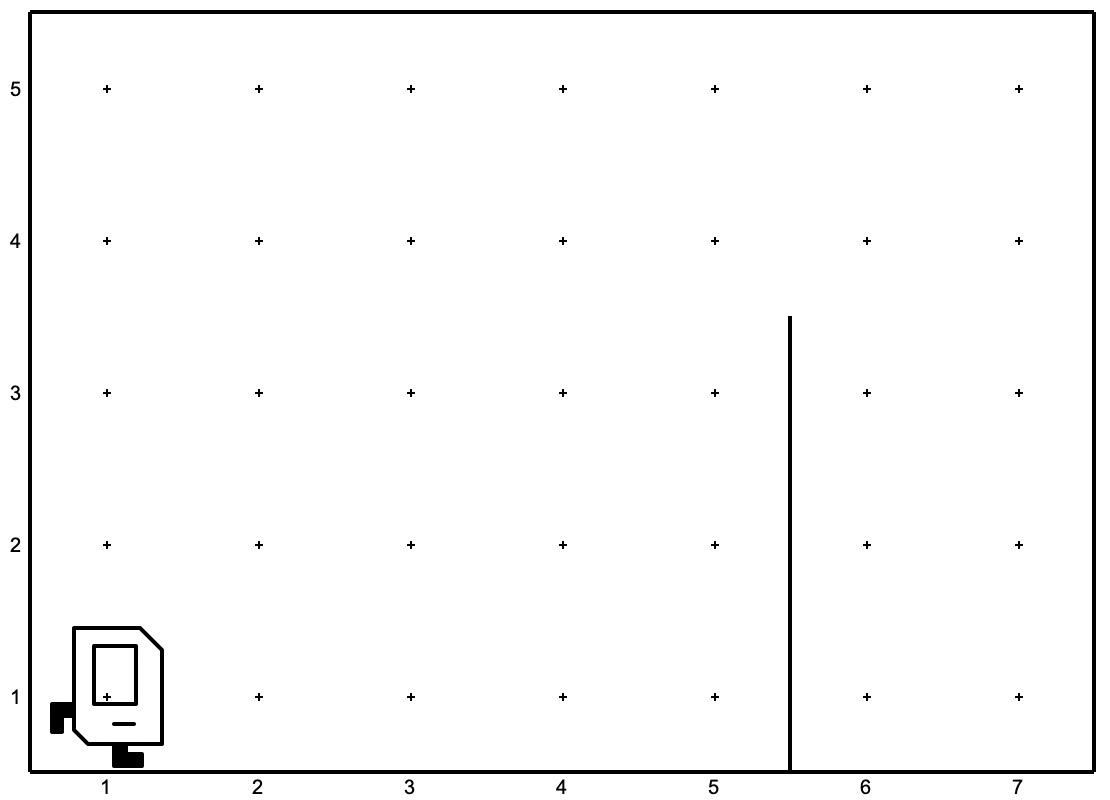
\includegraphics[scale=\figscale]{images/ch03/to_the_top/to_the_top_pre.jpg}
        \caption{မတိုင်မီ အခြေအနေ}   
        \label{fig:to_the_top_pre}
    \end{subfigure}
    \begin{subfigure}[t]{{\figpctw}\textwidth}
        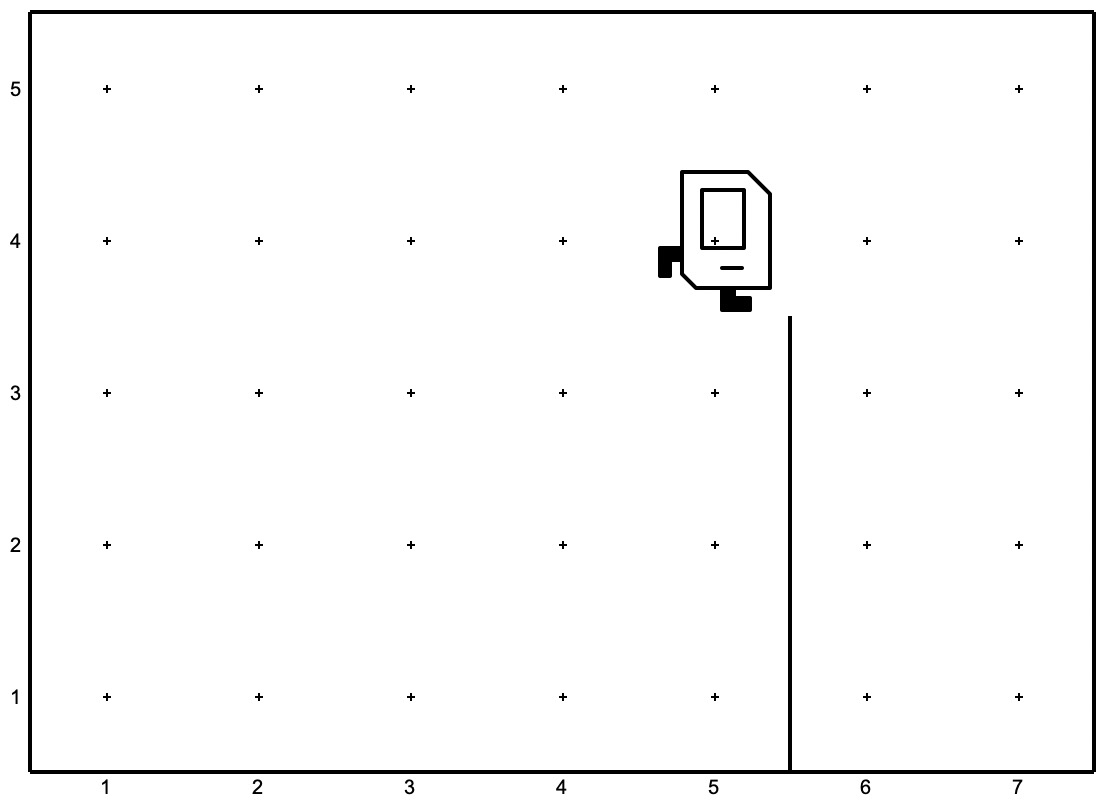
\includegraphics[scale=\figscale]{images/ch03/to_the_top/to_the_top_post.jpg}
        \caption{ပြီးနောက် အခြေအနေ} 
        \label{fig:to_the_top_post}   
    \end{subfigure}
    \caption{တိုင်ထိပ်သို့}
    \label{fig:to_the_top}
\end{figure}
%
တိုင်အောက်ခြေကိုသွားတာနဲ့ တိုင်ထိပ်တက်တာ အလုပ်နှစ်ခု ပါဝင်တယ်လို့ မြင်နိုင်တယ်။ ဒီအတွက် ဖန်ရှင်နှစ်ခု သတ်မှတ်ပေးပါမယ်။
%
\setlength{\fboxsep}{0pt}
\begin{minted}[frame=\mintframe, framerule=\mintrule,framesep= \mintsep, xleftmargin=\xlftmargin
    , bgcolor=mintbgcolor,rulecolor=mintrulecolor
    , python3=true,escapeinside=ßß]{python}
def go_to_pole():
    while front_is_clear():
        move()
\end{minted}
%
\betweenminted{\medskipamount}
%
\setlength{\fboxsep}{0pt}
\begin{minted}[frame=\mintframe, framerule=\mintrule,framesep= \mintsep, xleftmargin=\xlftmargin
    , bgcolor=mintbgcolor,rulecolor=mintrulecolor
    , python3=true,escapeinside=ßß]{python}
def ascend_pole():
    while right_is_blocked():
        move()
\end{minted}
%
အထက်ပါ ဖန်ရှင်နှစ်ခုနဲ့ \fCode{go\_to\_top} ကို ဆက်လက် သတ်မှတ်ပါမယ်
%
\setlength{\fboxsep}{0pt}
\begin{minted}[frame=\mintframe, framerule=\mintrule,framesep= \mintsep, xleftmargin=\xlftmargin
    , bgcolor=mintbgcolor,rulecolor=mintrulecolor
    , python3=true,escapeinside=ßß]{python}
def go_to_top():
    go_to_pole()
    turn_left()
    ascend_pole()
    turn_right()
\end{minted}
%
\fCode{go\_to\_pole} အပြီးမှာ ကားရဲလ်ဟာ တိုင်ခြေမှာ အရှေ့ဘက်မျက်နှာမူပြီး ရှိနေမှာပါ။ \fCode{ascend\_pole} က တိုင်ခြေမှာ ကားရဲလ် အပေါ်ဘက်ကို မျက်နှာမူတဲ့ အနေအထားကနေ စရပါမယ်။ \fCode{go\_to\_pole} ပြီးရင် \fCode{ascend\_pole} အတွက် အသင့်အနေအထားဖြစ်အောင် \fCode{turn\_left} လုပ်ပေးရပါမယ်။

ဖန်ရှင် စတင်မလုပ်ဆောင်မီ ကြိုတင်ရှိနေရမဲ့ အခြေအနေကို ပရီကွန်ဒီရှင်လို့ ပြောခဲ့ပါတယ်။ ဖန်ရှင် သတ်မှတ်တဲ့အခါ ပရီကွန်ဒီရှင်ကို တိတိကျကျ စဉ်းစားဖို့ လိုပါတယ်။ ဖန်ရှင်အသုံးပြုတဲ့အခါမှာလည်း သတ်မှတ်ထားတဲ့ ပရီကွန်ဒီရှင် အတိုင်းကိုက်ညီဖို့ လိုတယ်။ \fCode{ascend\_pole} ပရီကွန်ဒီးရှင်းဟာ တိုင်ခြေမှာ ကားရဲလ် အပေါ်ဘက်ကို မျက်နှာမူတဲ့ အနေအထား ဖြစ်ပါတယ်။ ပုံ \fRefNo{\ref{fig:mutp_pre_and_post}} (\fRefNo{\subref{fig:mutp_pre1}}) ကို ကြည့်ပါ။ %အကယ်၍ အဲဒီအတိုင်းမဟုတ်ရင် မက်သဒ်ကလည်း မှန်ကန်ကောင် လုပ်ဆောင်ပေးနိုင်ဖို့ မသေချာနိုင်ပါဘူး။

ဖန်ရှင် လုပ်ဆောင်အပြီးမှာ ရှိနေရမဲ့ အခြေအနေကို ပို့စ်ကွန်ဒီရှင်လို့ ဖော်ပြခဲ့တယ်။ ဖန်ရှင်တစ်ခုဟာ ပရီကွန်ဒီရှင်နဲ့ ကိုက်ညီတဲ့ အနေအထားကနေ စတင်ရင် ပို့စ်ကွန်ဒီရှင်နဲ့ ကိုက်ညီအောင်လုပ်ဆောင်ပေးပြီး အဆုံးသတ်ရမှာပါ။ ပုံ \fRefNo{\ref{fig:mutp_pre_and_post}} (\fRefNo{\subref{fig:mutp_post}}) မှာ \fCode{ascend\_pole} ပို့စ်ကွန်ဒီရှင်ကို တွေ့နိုင်ပါတယ်။
%
\begin{figure}[htb!]
    \hfuzz=100pt
    \newcommand{\figpctw}{0.52}
    \newcommand{\figscale}{0.165}
    \begin{subfigure}[t]{{\figpctw}\textwidth}
        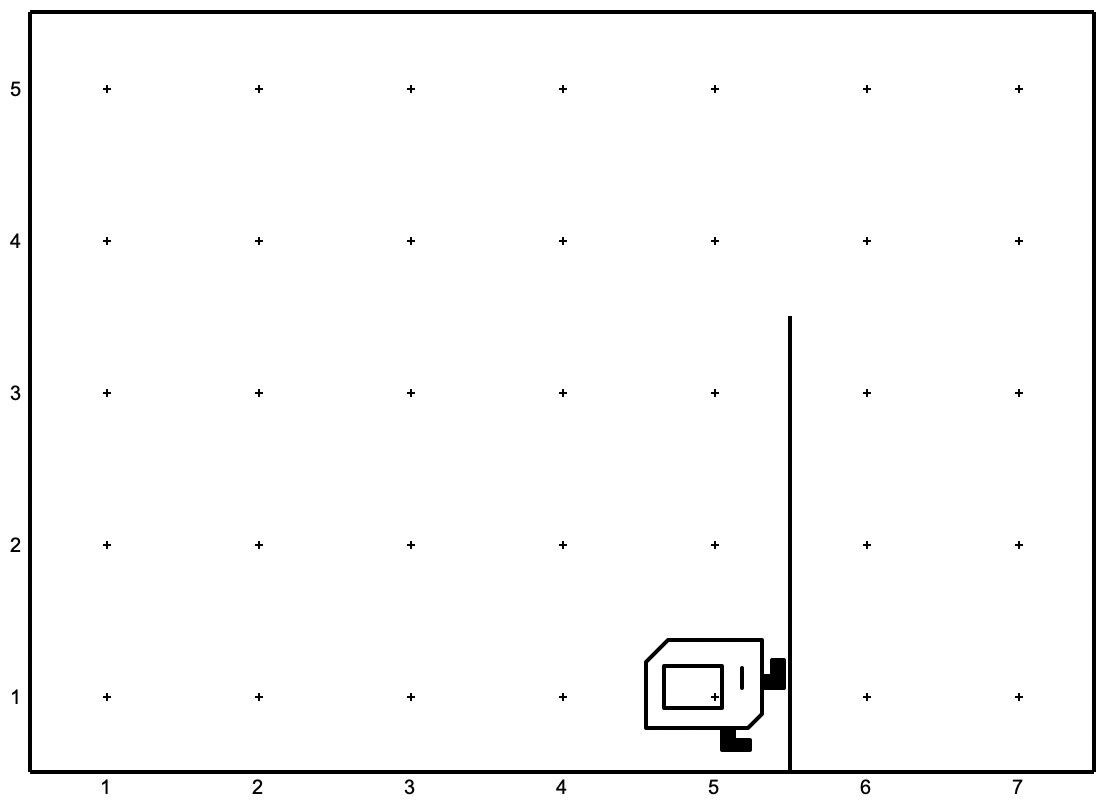
\includegraphics[scale=\figscale]{images/ch03/to_the_top/move_up_the_pole_pre1.jpg}
        \caption{}   
        \label{fig:mutp_pre1}
    \end{subfigure}
    \begin{subfigure}[t]{{\figpctw}\textwidth}
        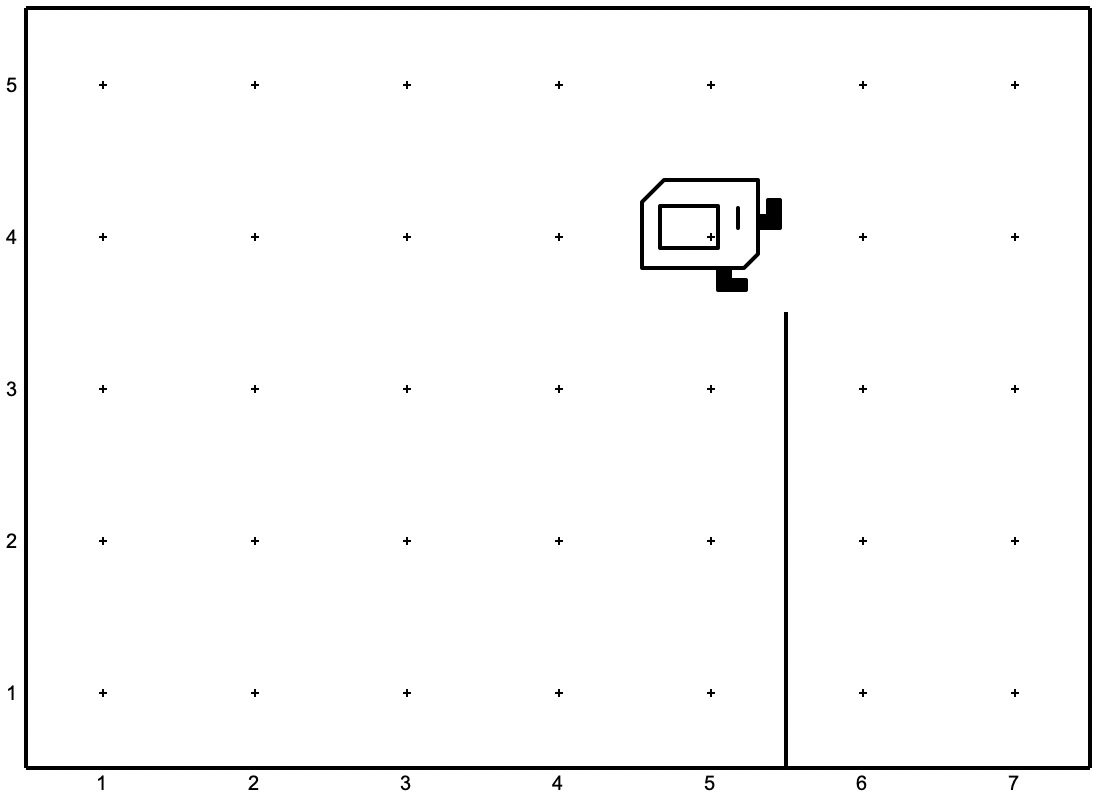
\includegraphics[scale=\figscale]{images/ch03/to_the_top/move_up_the_pole_post1.jpg}
        \caption{} 
        \label{fig:mutp_post}   
    \end{subfigure}
    \caption{\fCptCodeBf{ascend\_pole} ပရီကွန်ဒီးရှင်းနှင့် ပို့စ်ကွန်ဒီးရှင်း}
    \label{fig:mutp_pre_and_post}
\end{figure}


ဖန်ရှင် ပရီကွန်ဒီရှင် ပို့စ်ကွန်ဒီရှင်ကို သင့်တော်သလို သတ်မှတ်နိုင်ပါတယ်။ ပုံ (\fRefNo{\ref{fig:mutp_pre_and_post_v2}}) တွင် \fCode{ascend\_\allowbreak pole} အတွက် အခြား ရွေးချယ်နိုင်တဲ့ ပရီ နဲ့ ပို့စ် ကွန်ဒီရှင်ကို  ကြည့်ပါ။

\begin{figure}[tbh!]
    \hfuzz=100pt
    \newcommand{\figpctw}{0.52}
    \newcommand{\figscale}{0.165}
    \begin{subfigure}[t]{{\figpctw}\textwidth}
        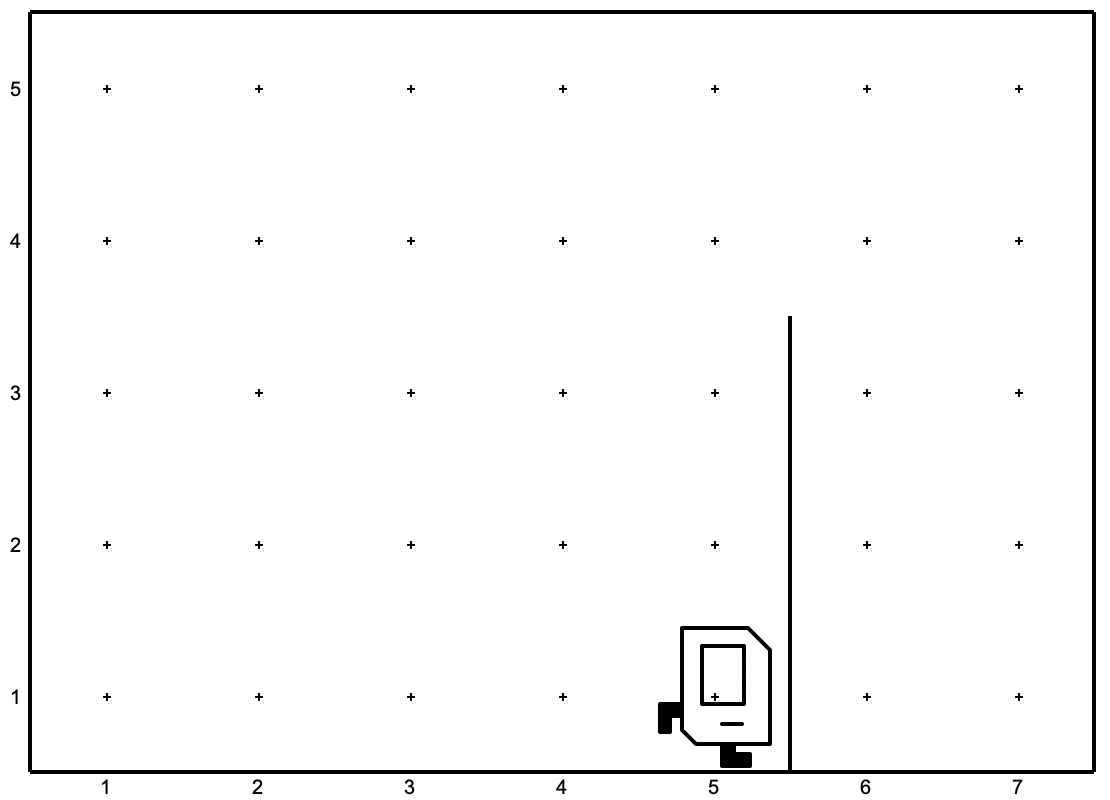
\includegraphics[scale=\figscale]{images/ch03/to_the_top/move_up_the_pole_pre_v2.jpg}
        \caption{}   
        \label{fig:mutp_pre_v2}
    \end{subfigure}
    \begin{subfigure}[t]{{\figpctw}\textwidth}
        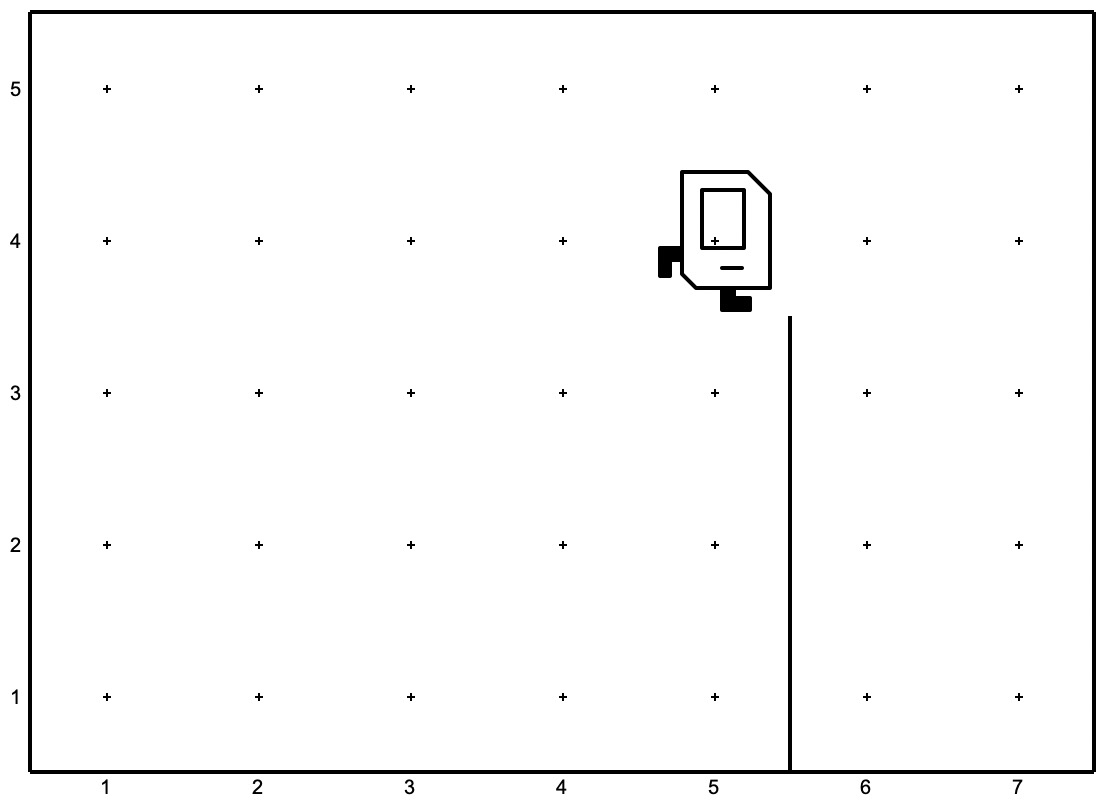
\includegraphics[scale=\figscale]{images/ch03/to_the_top/move_up_the_pole_post_v2.jpg}
        \caption{} 
        \label{fig:mutp_post_v2}   
    \end{subfigure}
    \caption{\fCptCodeBf{ascend\_pole} ပရီ နဲ့ ပို့စ် ကွန်ဒီရှင်}
    \label{fig:mutp_pre_and_post_v2}
\end{figure}

အထက်ပါ ပရီ နဲ့ ပို့စ် ကွန်ဒီရှင်အရ \fCode{ascend\_pole} ကို အခုလို 
%
\setlength{\fboxsep}{0pt}
\begin{minted}[frame=\mintframe, framerule=\mintrule,framesep= \mintsep, xleftmargin=\xlftmargin
    , bgcolor=mintbgcolor,rulecolor=mintrulecolor
    , python3=true,escapeinside=ßß]{python}
def ascend_pole():
    turn_left()
    while right_is_blocked():
        move()
    turn_right()
\end{minted}
%
သတ်မှတ်ရမှာပါ။ \fCode{go\_to\_top} ကလည်း ဒီလို ဖြစ်သွားမယ်
%
\setlength{\fboxsep}{0pt}
\begin{minted}[frame=\mintframe, framerule=\mintrule,framesep= \mintsep, xleftmargin=\xlftmargin
    , bgcolor=mintbgcolor,rulecolor=mintrulecolor
    , python3=true,escapeinside=ßß]{python}
def go_to_top():
    go_to_pole()
    ascend_pole()
\end{minted}
%

\section{ဖန်ရှင်များဖြင့် abstraction များ တည်ဆောက်ခြင်း}
အခန်း (\fRefNo{\ref{ch:ch02}}) စာမျက်နှာ (\fRefNo{\pageref{lst:repair_street}}) မှ လမ်းပြင်တဲ့ ပရိုဂရမ်မှာ ကွန်နာတစ်ခုဟာ ဘိပါလည်းမရှိ၊ အောက်ဘက်ကပ်လျက် နံရံလည်းမရှိရင်  ဘိပါတစ်ခု ချထားပေးရပါတယ်။ ဒီကိစ္စ ဆောင်ရွက်ပေးဖို့အတွက် ဖန်ရှင်တစ်ခု သတ်မှတ်နိုင်ပါတယ်။ 
%
\begin{figure}[htb!]
    {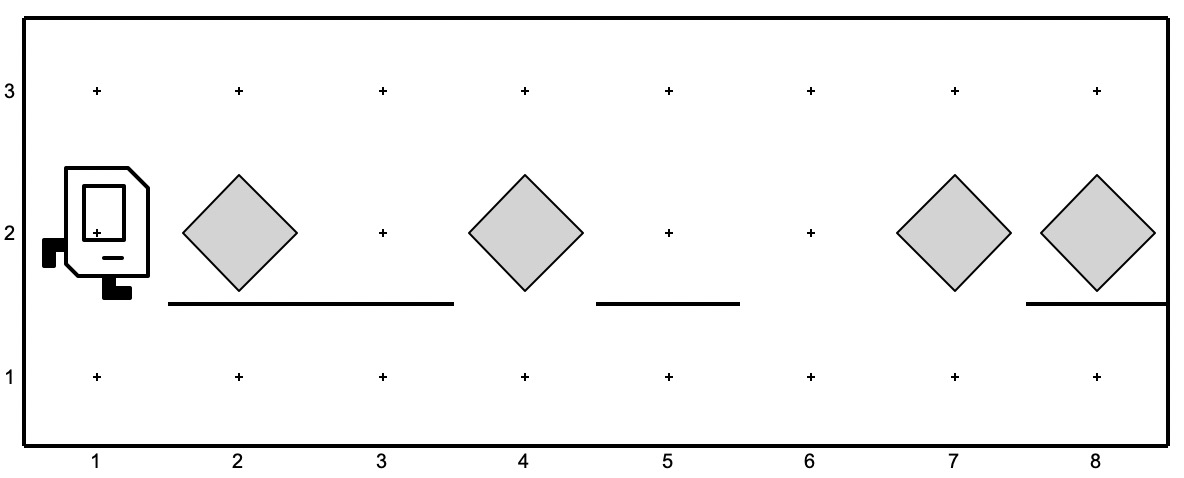
\includegraphics[width=0.5\linewidth]{images/ch02/st_repair/init.jpg}}
    \caption{}
\end{figure}
%
%
\setlength{\fboxsep}{0pt}
\begin{minted}[frame=\mintframe, framerule=\mintrule,framesep= \mintsep, xleftmargin=\xlftmargin
    , bgcolor=mintbgcolor,rulecolor=mintrulecolor
    , python3=true,escapeinside=ßß]{python}
def repair_corner():
    if right_is_clear():
        if no_beepers_present():
            put_beeper()
\end{minted}
%
အခြေအနေနှစ်ခုစလုံး မှန်တော့မှ ဘိပါချပေးဖို့ \fEn{nested} \fCode{if}  သုံးထားတာက နားလည်ရ အတန်အသင့် ခက်ခဲနိုင်ပါတယ်။  ဒါပေမဲ့ \fCode{repair\_corner} ကို အသုံးပြုတဲ့အခါ ဘယ်လိုရေးထားလဲ စဉ်းစားစရာ မလိုပါဘူး။ ဘိပါလည်းမရှိ၊ ညာဘက် နံရံလည်းမရှိတဲ့ ကွန်နာမှာ ဘိပါချချင်ရင် \fCode{repair\_corner} ဖန်ရှင်နဲ့ လုပ်လို့ရတယ်ဆိုတာ သိထားရင် သုံးလို့ရပြီ။

ဖန်ရှင် သတ်မှတ်တဲ့အခါ ဆောင်ရွက်ပေးစေချင်တဲ့ ကိစ္စကို ‘ဘယ်လို လုပ်ရမှာလဲ’ အသေးစိတ် စဉ်းစားရမှာဖြစ်ပေမဲ့ အသုံးပြုတဲ့အခါမှာတော့ ဒီလိုအသေးစိတ်တွေကို ထပ်ပြီး စဉ်းစားဖို့ မလိုတော့ပါဘူး။ ဖန်ရှင် ‘ဘာလုပ်ပေးတာလဲ’ ကပဲ အရေးကြီးတယ်။ ‘ဘယ်လို’ တည်ဆောက်ထားလဲ သိစရာမလိုဘဲ ‘ဘာ’ လုပ်ပေးလဲ သိရုံနဲ့ အသုံးပြုလို့ရစေတာကို \fEn{abstraction} လုပ်တယ်လို့ခေါ်ပါတယ်။ \fEn{Abstraction} လုပ်ခြင်းအတွက် ဖန်ရှင်တွေဟာ အဓိက အကျဆုံး အခြေခံ အုတ်ချပ်တွေပါပဲ။ 


\fEn{Abstraction} လုပ်ထားလိုက်ခြင်းအားဖြင့် ရှုပ်ရှုပ်ထွေးထွေးတွေ ထပ်ခါထပ်ခါ ခေါင်းရှုပ်ခံ စဉ်းစားနေဖို့ မလိုအပ်တော့ဘဲ ကိစ္စတစ်ခုကို အလွယ်တကူ လုပ်ဆောင်လို့ရသွားတယ်။ ကုဒ်တွေဖတ်ရတာလည်း ပိုရှင်းပြီး နားလည်ရ လွယ်ကူသွားတယ်။ ဒါကြောင့် ပရိုဂရမ်တွေ တည်ဆောက်ရာမှာ \fEn{abstraction} လုပ်ခြင်းဟာ အရေးပါပါတယ်။ အရေးကြီးဆုံးလို့ ဆိုရင်လည်း မမှားဘူး။  ကြီးမားရှုပ်ထွေးတဲ့ ဆော့ဖ်ဝဲတွေကို လေ့လာကြည့်ရင်  \fEn{abstraction} ပေါင်းများစွာနဲ့ တစ်ဆင့်ပြီးတစ်ဆင့်၊ တစ်လွှာပြီးတစ်လွှာ တည်ဆောက်ထားတယ်ဆိုတာ တွေ့ရမှာပါ။

\fCode{repair\_corner} ဟာ အနိမ့်ဆုံးအလွှာက အခြေခံ \fEn{abstraction} တစ်ခု ဖြစ်တယ် ဆိုပါစို့။ ၎င်းကို အခြေခံပြီး တစ်ဆင့်ပိုမြင့်တဲ့ အလွှာအတွက် \fEn{abstraction} တွေကို တည်ဆောက်ယူနိုင်ပါတယ်။ ဥပမာ
%
\setlength{\fboxsep}{0pt}
\begin{minted}[frame=\mintframe, framerule=\mintrule,framesep= \mintsep, xleftmargin=\xlftmargin
    , bgcolor=mintbgcolor,rulecolor=mintrulecolor
    , python3=true,escapeinside=ßß]{python}
def repair_street():
    while front_is_clear():
        repair_corner()
    repair_corner()
\end{minted}
%
ဒီအလွှာထက် နောက်ထပ် တစ်ဆင့်ပိုမြင့်တဲ့ \fEn{abstraction} တွေကိုလည်း ဆက်လက် တည်ဆောက်ယူနိုင်ပါတယ်။ ဥပမာ \fCode{repair\_world} ကို တည်ဆောက်ရာမှာ \fCode{repair\_street} ကို အခြေခံအစိတ်အပိုင်းအဖြစ် အသုံးပြုနိုင်ပါတယ်။ ဒီလို \fEn{abstraction} အလွှာတွေ အဆင့်ဆင့်နဲ့ ပရိုဂရမ် တည်ဆောက်နည်း တွေကို ဆက်လက်လေ့လာကြရပါမယ်။


\section{Bottom-up Programming}

ကြီးကျယ်ခမ်းနားတဲ့ အဆောက်အအုံကြီးတွေ၊ လျှို့ဝှက်ဆန်းကြယ်တဲ့ သဘာဝဖြစ်စဉ်တွေ၊ အံ့ဖွယ်သိပ္ပံနှင့် နည်းပညာ ဆန်းသစ်တီထွင်မှုတွေ စတဲ့အရာတွေအားလုံးဟာ ရိုးရှင်းတဲ့ အစိတ်အပိုင်းလေးတွေနဲ့ ဖွဲ့စည်းထားတာပါပဲ။ ဒါကြောင့် အရွယ်အစား ကြီးမား ရှုပ်ထွေးတဲ့ ပရိုဂရမ်တွေကိုလည်း ရိုးရှင်းတဲ့ အစိတ်အပိုင်းလေးတွေနဲ့ အခြေပြု ဖွဲ့စည်းတည်ဆောက်သင့်တယ်လို့ ယူဆမယ်ဆိုရင် ကျိုးကြောင်းဆီလျော်တယ်ပဲ ဆိုရမှာပါ။

ခက်ခဲရှုပ်ထွေးတဲ့ ကိစ္စတစ်ခုကို ဖြေရှင်းတဲ့အခါ အပိုင်းတွေခွဲပြီး တစ်ပိုင်းချင်းကို သီးခြားဖြေရှင်းလေ့ရှိတယ်။ အပိုင်းတွေခွဲလိုက်ခြင်းအားဖြင့် တစ်ပိုင်းစီဟာ မူလဖြေရှင်းရမဲ့ ကိစ္စလောက် မခက်ခဲတော့ပါဘူး။ အရွယ်အစားအားဖြင့်လည်း နဂိုထက် ငယ်သွားမယ်။ အပိုင်း တစ်ပိုင်းချင်းစီကို ဖြေရှင်းတဲ့အခါမှာလည်း အလားတူပဲ လုပ်ဆောင်နိုင်တယ်။ အပိုင်းတစ်ပိုင်းကို သူ့ထက်သေးငယ်တဲ့ အပိုင်းတွေအဖြစ် ထပ်မံခွဲထုတ်နိုင်ပါတယ်။ ဒီတိုင်း တစ်ဆင့်ပြီးတစ်ဆင့် လုပ်သွားမယ်ဆိုရင် နောက်ဆုံးမှာ အလွယ်တကူဖြေရှင်းလို့ရတဲ့ အစိတ်အပိုင်းလေးတွေ ဖြစ်သွားရမှာပါပဲ။ \fEnEmp{Bottom-up programming} ဆိုတာကတော့ ပရိုဂရမ်ရေးပြီး ကိစ္စတစ်ခုကို ဖြေရှင်းရာမှာ ရိုးရှင်းသထက်ရိုးရှင်း၊ သေးငယ်သထက်သေးငယ်တဲ့ အပိုင်းလေးတွေဖြစ်လာအောင် အဆင့်ဆင့်ပိုင်းခွဲပြီး အောက်ခြေအရိုးရှင်းဆုံးအလွှာကနေ အပေါ်ကိုတစ်ဆင့်ချင်းတက် ဖြေရှင်းတဲ့နည်း ဖြစ်တယ်။ လေ့လာကြည့်ကြရအောင်။

ပုံ (\fRefNo{\ref{fig:hurdle_jumping_init}}) ကမ္ဘာမှာ ကားရဲလ် တန်းကျော်ပြေးပြိုင်ရပါမယ်။ ထောင်လိုက်နံရံတွေကို တန်းတွေလို့ယူဆပါ။ တန်းတွေဟာ အနိမ့်အမြင့် အမျိုးမျိုးဖြစ်နိုင်ပါတယ်။ ကမ္ဘာရဲ့ အပေါ်ဘက် နံရံကို ထိတဲ့အထိတော့ မြင့်လို့မရပါဘူး။ ဒါမှ တန်းကိုကျော်ပြီး အခြားဘက်ကို သွားလို့ရမှာပါ။ \((1, 1)\) ကွန်နာကနေ တာစထွက်မှာဖြစ်ပြီး \((14, 1)\) မှာ ပန်းဝင်ရမှာပါ။
%
\begin{figure}[htb!]
    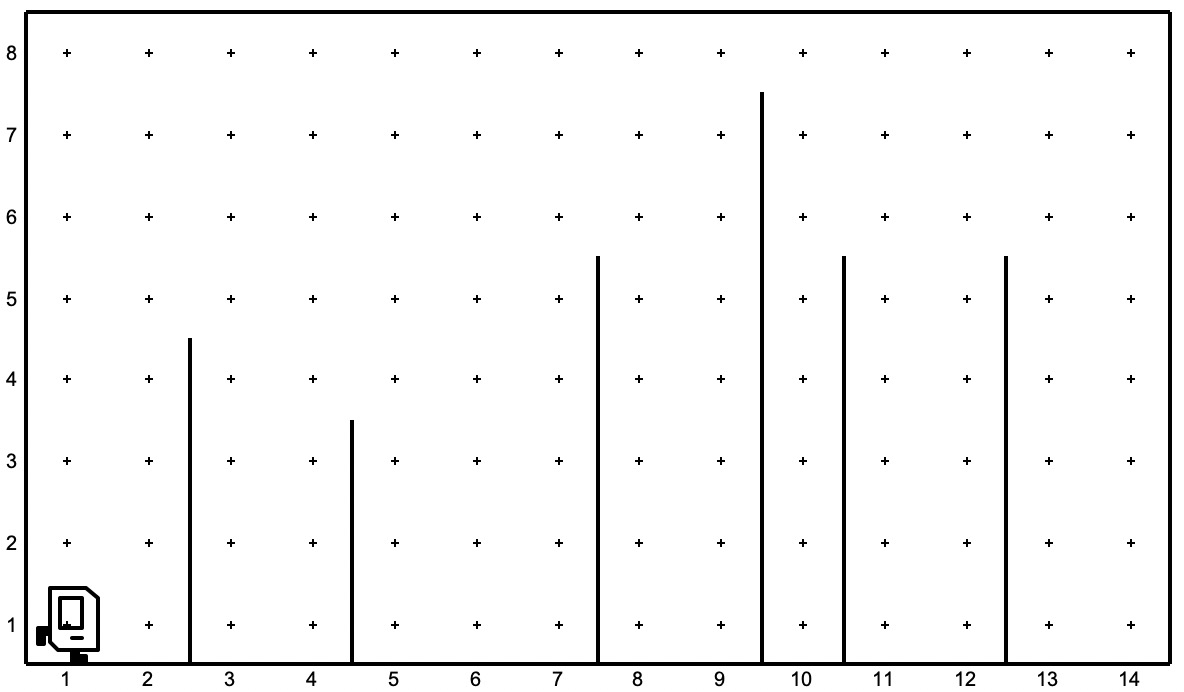
\includegraphics[width=4.5in]{images/ch03/hurdle_jumping/init_w1.jpg}
    \caption{}
    \label{fig:hurdle_jumping_init}
\end{figure}
%

တန်းကျော်ပြေးတဲ့ ကိစ္စမှာ ပါဝင်တဲ့ အပိုင်းတစ်ခုက တန်းတစ်ခုကျော်တာ။ တန်းတစ်ခု ကျော်တာကို ထပ်ခွဲကြည့်ရင် အပေါ်တက်တာနဲ့ အောက်ဆင်းတာ နှစ်ပိုင်းရှိမယ်။ အခုလို နဂိုမူလကိစ္စတစ်ခုကနေ တစ်ဆင့်ထက်တစ်ဆင့် ပိုသေးငယ်တဲ့ အပိုင်းလေးတွေဖြစ်လာအောင် ခွဲထုတ်တာကို \fEnEmp{problem decomposition} လုပ်တယ်လို ခေါ်ပါတယ်။ 

\fEn{Bottom-up programming} နည်းနဲ့ ပရိုဂရမ်ရေးတဲ့အခါ \fEn{problem decomposition} အရင်ဦးဆုံး  လုပ်ရတယ်။ ပြီးရင် အောက်ဆုံးအလွှာမှ အသေးဆုံးအပိုင်းလေးတွေကနေ စတင်ဖြေရှင်းတယ်။ ပြီးတဲ့အခါ အဲဒီ အသေးဆုံး အပိုင်းလေးတွေကို အခြေခံအစိတ်အပိုင်းအဖြစ် အသုံးပြုပြီး  အောက်ဆုံးအလွှာထက် တစ်ဆင့်မြင့်တဲ့ အပေါ်အလွှာက အပိုင်းတွေကို ဆက်လက်ဖြေရှင်းတယ်။ ဒီအလွှာက အပိုင်းတွေကို  အခြေခံအစိတ်အပိုင်းအဖြစ် အသုံးပြုပြီး နောက်ထပ်တစ်ဆင့် ပိုမြင့်တဲ့အလွှာက အပိုင်းတွေကို ဆက်လက်ဖြေရှင်းမှာဖြစ်တယ်။ ဒီလိုမျိုး အောက်ကနေ အပေါ်ကို တစ်လွှာပြီးတစ်လွှာ တက်သွားပြီး ဖြေရှင်းတဲ့ နည်းစနစ်ဟာ \fEn{bottom-up programming} ပါပဲ။ 

တန်းကျော်ပြေးပွဲမှာ \fEn{Problem Decomposition} လုပ်ထားတာကို တစ်လွှာချင်း ခွဲကြည့်မယ်ဆိုရင် အခုလိုတွေ့ရမှာ ဖြစ်ပါတယ်။
%
\begin{itemize}
  \item တန်းကျော်ပြေးပြိုင်ပွဲဝင်ခြင်း
  \begin{itemize}
    \item တန်းတစ်ခုကျော်ခြင်း
    \begin{itemize}
      \item အပေါ်တက်ခြင်း
      \item အောက်ဆင်းခြင်း
    \end{itemize}
  \end{itemize} 
\end{itemize}
%
\fEn{Bottom-up} နည်းအရ အောက်ဆုံးအလွှာ အပေါ်တက်၊ အောက်ဆင်း ကိစ္စကို ပထမဆုံး ဖြေရှင်းပါမယ်။ အပိုင်းတစ်ခုအတွက် ဖန်ရှင်တစ်ခု သတ်မှတ်ရပါမယ်။

%
\setlength{\fboxsep}{0pt}
\begin{minted}[frame=\mintframe, framerule=\mintrule,framesep= \mintsep, xleftmargin=\xlftmargin
    , bgcolor=mintbgcolor,rulecolor=mintrulecolor
    , python3=true,escapeinside=ßß]{python}
def ascend():
    ß\PYG{l+s+sd}{\PYGZdq{}\PYGZdq{}\PYGZdq{}}ß
    ß\PYG{l+s+sd}{\fMM{တန်းနဲ့လွတ်တဲ့အထိ အပေါ်သို့ တက်သည်}}ß
    ß\PYG{l+s+sd}{\fEnEmp{Precondition:} \fMM{တန်းဘယ်ဘက် ခြေရင်းမှာ အရှေ့ဘက်မျက်နှာမူပြီး ရှိနေ}}ß
    ß\PYG{l+s+sd}{\fEnEmp{Postcondition:} \fMM{တန်းထိပ်အပေါ် ဘယ်ဘက်ကွန်နာမှာ အရှေ့ဘက်မျက်နှာမူပြီး ရှိနေ}}ß
    ß\PYG{l+s+sd}{\PYGZdq{}\PYGZdq{}\PYGZdq{}}ß
    turn_left()
    while right_is_blocked():
        move()
    turn_right()
\end{minted}
%
\betweenminted{\medskipamount}
%
\setlength{\fboxsep}{0pt}
\begin{minted}[frame=\mintframe, framerule=\mintrule,framesep= \mintsep, xleftmargin=\xlftmargin
    , bgcolor=mintbgcolor,rulecolor=mintrulecolor
    , python3=true,escapeinside=ßß]{python}
def descend():
    ß\PYG{l+s+sd}{\PYGZdq{}\PYGZdq{}\PYGZdq{}}ß
    ß\PYG{l+s+sd}{\fMM{တန်းအောက်သို့ ပြန်ဆင်းသည်}}ß
    ß\PYG{l+s+sd}{\fEnEmp{Precondition:} \fMM{တန်းထိပ်အပေါ် ညာဘက်ကွန်နာမှာ အရှေ့ဘက်မျက်နှာမူပြီး ရှိနေ}}ß
    ß\PYG{l+s+sd}{\fEnEmp{Postcondition:} \fMM{တန်းညာဘက် ခြေရင်းမှာ အရှေ့ဘက်မျက်နှာမူပြီး ရှိနေ}}ß
    ß\PYG{l+s+sd}{\PYGZdq{}\PYGZdq{}\PYGZdq{}}ß
    turn_right()
    while front_is_clear():
        move()
    turn_left()
\end{minted}
%

အထက်ပါ ဖန်ရှင်နှစ်ခုကို အသုံးပြုပြီး အပေါ်တစ်ဆင့် ပိုမြင့်တဲ့ အလွှာက တန်းတစ်ခုကျော်တာကို ဆက်လက်ဖြေရှင်းရပါမယ်။ \fCode{ascend} နဲ့ \fCode{descend} ပရီနဲ့ ပို့စ် ကွန်ဒီရှင်တွေအရ \fCode{move} လုပ်ပေးဖို့လိုပါတယ်။
%
\setlength{\fboxsep}{0pt}
\begin{minted}[frame=\mintframe, framerule=\mintrule,framesep= \mintsep, xleftmargin=\xlftmargin
    , bgcolor=mintbgcolor,rulecolor=mintrulecolor
    , python3=true,escapeinside=ßß]{python}
def jump_over_hurdle():
    ß\PYG{l+s+sd}{\PYGZdq{}\PYGZdq{}\PYGZdq{}}ß
    ß\PYG{l+s+sd}{\fMM{တန်းတစ်ခုကို ကျော်သည်}}ß
    ß\PYG{l+s+sd}{\fEnEmp{Precondition:} \fMM{တန်းဘယ်ဘက် ခြေရင်းမှာ အရှေ့ဘက်မျက်နှာမူပြီး ရှိနေ}}ß
    ß\PYG{l+s+sd}{\fEnEmp{Postcondition:} \fMM{တန်းညာဘက် ခြေရင်းမှာ အရှေ့ဘက်မျက်နှာမူပြီး ရှိနေ}}ß
    ß\PYG{l+s+sd}{\PYGZdq{}\PYGZdq{}\PYGZdq{}}ß
    ascend()
    move()
    descend()
\end{minted}
%

ဒီဖန်ရှင်နဲ့ နောက်တစ်ဆင့်ကို ဆက်လက်တည်ဆောက်ရပါမယ်။ ရှေ့မှာရှင်းနေလျှင် ရှေ့တိုးမယ်၊ မရှင်းလျှင် တန်းကိုကျော်ရမယ်။ ပန်းဝင်ဖို့အတွက်ဆိုလျှင် ဒီအလုပ်ကို ဆယ့်သုံးခါလုပ်ပေးရုံပါပဲ။
%
\setlength{\fboxsep}{0pt}
\begin{minted}[frame=\mintframe, framerule=\mintrule,framesep= \mintsep, xleftmargin=\xlftmargin
    , bgcolor=mintbgcolor,rulecolor=mintrulecolor
    , python3=true,escapeinside=ßß]{python}
def compete_hurdle_race():
    ß\PYG{l+s+sd}{\PYGZdq{}\PYGZdq{}\PYGZdq{}}ß
    ß\PYG{l+s+sd}{\fMM{တန်းကျော်ပြေးပြိုင်ပွဲ ပန်းဝင်သည်ထိ ယှဉ်ပြိုင်သည်}}ß
    ß\PYG{l+s+sd}{\fEnEmp{Precondition:} \fMM{(၁,၁) ကွန်နာတွင် အရှေ့ဘက်မျက်နှာမူနေ}}ß
    ß\PYG{l+s+sd}{\fEnEmp{Postcondition:} \fMM{(၁၄,၁) ကွန်နာတွင် အရှေ့ဘက်မျက်နှာမူနေ}}ß
    ß\PYG{l+s+sd}{\PYGZdq{}\PYGZdq{}\PYGZdq{}}ß
    for i in range(13):
        if front_is_clear():
            move()
        else:
            jump_over_hurdle()
\end{minted}
%

ပရိုဂရမ် အစအဆုံးကို လေ့လာကြည့်ပါ။ ဖန်ရှင်တစ်ခုချင်း ပရီနဲ့ ပို့စ် ကွန်ဒီရှင်တွေကို တိတိကျကျ မြင်အောင် ဂရုစိုက်ကြည့်ဖို့လည်း အရေးကြီးတယ်။ ဖန်ရှင် \fEn{docstring} မှာ ၎င်းဖန်ရှင် ပရီနဲ့ ပို့စ် ကွန်ဒီရှင်ကို တိတိကျကျ ဖော်ပြထားတာဟာ အလေ့အထကောင်း တစ်ခုပါ။ ဖန်ရှင်တိုင်းမှာ ပါသင့်တယ်။

%
\setlength{\fboxsep}{0pt}
\begin{minted}[frame=\mintframe, framerule=\mintrule,framesep= \mintsep, xleftmargin=\xlftmargin
    , bgcolor=mintbgcolor,rulecolor=mintrulecolor
    , python3=true,escapeinside=ßß]{python}
# File: hurdle_jumping.py
from stanfordkarel import *


def main():
    """Hurdle Jumping Program"""
    compete_hurdle_race()


def ascend():
    ß\PYG{l+s+sd}{\PYGZdq{}\PYGZdq{}\PYGZdq{}}ß
    ß\PYG{l+s+sd}{\fMM{တန်းနဲ့လွတ်တဲ့အထိ အပေါ်သို့ တက်သည်}}ß
    ß\PYG{l+s+sd}{\fEnEmp{Precondition:} \fMM{တန်းဘယ်ဘက် ခြေရင်းမှာ အရှေ့ဘက်မျက်နှာမူပြီး ရှိနေ}}ß
    ß\PYG{l+s+sd}{\fEnEmp{Postcondition:} \fMM{တန်းထိပ်အပေါ် ဘယ်ဘက်ကွန်နာမှာ အရှေ့ဘက်မျက်နှာမူပြီး ရှိနေ}}ß
    ß\PYG{l+s+sd}{\PYGZdq{}\PYGZdq{}\PYGZdq{}}ß
    turn_left()
    while right_is_blocked():
        move()
    turn_right()


def descend():
    ß\PYG{l+s+sd}{\PYGZdq{}\PYGZdq{}\PYGZdq{}}ß
    ß\PYG{l+s+sd}{\fMM{တန်းအောက်သို့ ပြန်ဆင်းသည်}}ß
    ß\PYG{l+s+sd}{\fEnEmp{Precondition:} \fMM{တန်းထိပ်အပေါ် ညာဘက်ကွန်နာမှာ အရှေ့ဘက်မျက်နှာမူပြီး ရှိနေ}}ß
    ß\PYG{l+s+sd}{\fEnEmp{Postcondition:} \fMM{တန်းညာဘက် ခြေရင်းမှာ အရှေ့ဘက်မျက်နှာမူပြီး ရှိနေ}}ß
    ß\PYG{l+s+sd}{\PYGZdq{}\PYGZdq{}\PYGZdq{}}ß
    turn_right()
    while front_is_clear():
        move()
    turn_left()


def jump_over_hurdle():
    ß\PYG{l+s+sd}{\PYGZdq{}\PYGZdq{}\PYGZdq{}}ß
    ß\PYG{l+s+sd}{\fMM{တန်းတစ်ခုကို ကျော်သည်}}ß
    ß\PYG{l+s+sd}{\fEnEmp{Precondition:} \fMM{တန်းဘယ်ဘက် ခြေရင်းမှာ အရှေ့ဘက်မျက်နှာမူပြီး ရှိနေ}}ß
    ß\PYG{l+s+sd}{\fEnEmp{Postcondition:} \fMM{တန်းညာဘက် ခြေရင်းမှာ အရှေ့ဘက်မျက်နှာမူပြီး ရှိနေ}}ß
    ß\PYG{l+s+sd}{\PYGZdq{}\PYGZdq{}\PYGZdq{}}ß
    ascend()
    move()
    descend()


def compete_hurdle_race():
    ß\PYG{l+s+sd}{\PYGZdq{}\PYGZdq{}\PYGZdq{}}ß
    ß\PYG{l+s+sd}{\fMM{တန်းကျော်ပြေးပြိုင်ပွဲ ပန်းဝင်သည်ထိ ယှဉ်ပြိုင်သည်}}ß
    ß\PYG{l+s+sd}{\fEnEmp{Precondition:} \fMM{(၁,၁) ကွန်နာတွင် အရှေ့ဘက်မျက်နှာမူနေ}}ß
    ß\PYG{l+s+sd}{\fEnEmp{Postcondition:} \fMM{(၁၄,၁) ကွန်နာတွင် အရှေ့ဘက်မျက်နှာမူနေ}}ß
    ß\PYG{l+s+sd}{\PYGZdq{}\PYGZdq{}\PYGZdq{}}ß
    for i in range(13):
        if front_is_clear():
            move()
        else:
            jump_over_hurdle()


def turn_right():
    for i in range(3):
        turn_left()


if __name__ == "__main__":
    run_karel_program("hurdle_jumping")

\end{minted}
%


\subsection*{အမှိုက်သိမ်းတဲ့ ကားရဲလ်}
အခုတစ်ခါမှာ ကားရဲလ်က အမှိုက်တွေရှင်းပေးရပါမယ်။ ပုံ (\fRefNo{\ref{fig:stw}}) နမူနာ ကမ္ဘာမှာ ကြုံရာကျပန်း \fEn{(random)} ပြန့်ကျဲနေတဲ့ ဘိပါတွေကို အမှိုက်လို့ ယူဆပါ။  ကမ္ဘာအရွယ်အစား အမျိုးမျိုးအတွက် အမှိုက်ရှင်းပေးတဲ့ ပရိုဂရမ်တစ်ခု ရေးပေးရမှာပါ။
\begin{figure}[htb!]
    {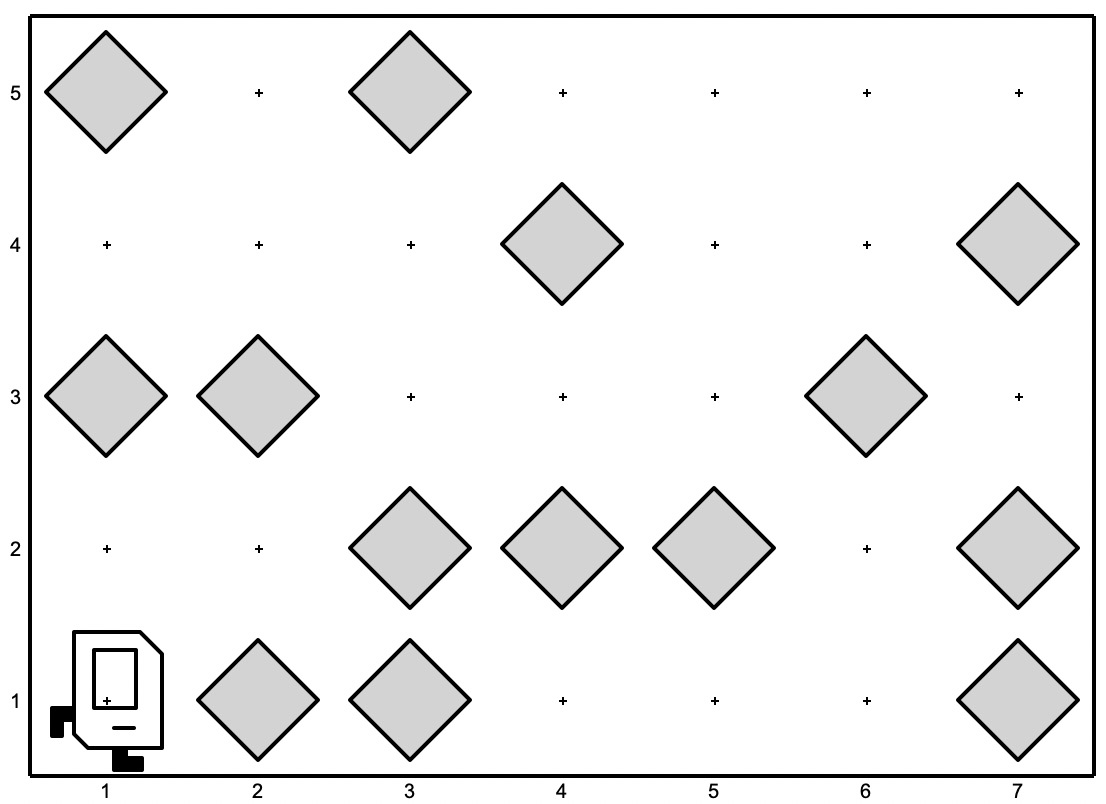
\includegraphics[width=.5\linewidth]{images/ch03/clean_the_world/init_w1.jpg}}
\caption{}
\label{fig:stw}
\end{figure}

ဒီကိစ္စကို ဖြေရှင်းဖို့က နည်းလမ်းတစ်ခုတည်း ရှိတာ မဟုတ်ပါဘူး။ နည်းလမ်းတစ်ခုက ဒီလိုပါ။ (၁) လမ်းကနေ စပြီး ရှင်းတယ် $\big\llbracket$စာမျက်နှာ \fRefNo{\pageref{fig:stw_alg1}} ပုံ (\fRefNo{\ref{fig:stw_alg1}}) (က) နှင့် (ခ) တွင် ကြည့်ပါ$\big\rrbracket$။ ပြီးရင် မြောက်ဘက် လှည့်ထားမယ် $\big\llbracket$ပုံ (\fRefNo{\ref{fig:stw_alg1}}) (ဂ)$\big\rrbracket$။ ရှင်းနေသေးတယ်ဆိုရင် ဒုတိယလမ်းကို တက်၊ အနောက်ဘက် မျက်နှာမူထားမယ် $\big\llbracket$ပုံ (\fRefNo{\ref{fig:stw_alg1}}) (ဃ)$\big\rrbracket$။ ဒုတိယလမ်းကို ဆက်ရှင်းပြီးတော့လည်း မြောက်ဘက်ကိုပဲ မျက်နှာမူထားပါမယ် $\big\llbracket$ပုံ (\fRefNo{\ref{fig:stw_alg1}}) (င)၊ (စ)$\big\rrbracket$။ ရှင်းနေသေးရင် တတိယလမ်းကို ကူး၊ အရှေ့ဘက်မျက်နှာ မူထားမယ် $\big\llbracket$ပုံ (\fRefNo{\ref{fig:stw_alg1}}) (ဆ)$\big\rrbracket$။ ဒီအတိုင်း တစ်လမ်းပြီးတစ်လမ်း ရှင်းသွားမှာဖြစ်တယ်။ လမ်းတစ်လမ်းရှင်းပြီး မြောက်ဘက်မျက်နှာမူလို့ ပိတ်နေရင် နောက်ထပ် လမ်းမရှိတော့ဘူး။ လမ်းအားလုံး ရှင်းပြီးသွားပြီ။ စာမျက်နှာ \fRefNo{\pageref{fig:stw_alg1_last_st}} ပုံ (\fRefNo{\ref{fig:stw_alg1_last_st}}) (က)၊ (ခ)၊ (ဂ) တို့ကို ကြည့်ပါ။ \fEn{Problem decomposition} လုပ်ကြည့်ရင် အောက်ပါအတိုင်း တွေ့နိုင်ပါတယ်။ 

%
\begin{figure}[htb!]
    \hfuzz=100pt
    \newcommand{\figpctw}{0.52}
    \newcommand{\figscale}{0.165}
    \begin{subfigure}[t]{{\figpctw}\textwidth}
        %\adjincludegraphics[width=2.5in,trim={0 0 0 {.55\height}}, clip, left]{ch03/SweepTheStreets/init_w1.jpg}
        \adjincludegraphics[scale=\figscale, trim={0 3pt 0 10cm}, clip, left]{images/ch03/clean_the_world/alg1/stp1a.jpg}
        \caption{}
        \label{fig:fst_bef}
    \end{subfigure}
    \begin{subfigure}[t]{{\figpctw}\textwidth}
        \adjincludegraphics[scale=\figscale, trim={0 3pt 0 10cm}, clip, left]{images/ch03/clean_the_world/alg1/stp1b.jpg}
        \caption{}
        \label{fig:fst_aft}
    \end{subfigure}

    \begin{subfigure}[t]{{\figpctw}\textwidth}
        \adjincludegraphics[scale=\figscale, trim={0 3pt 0 10cm}, clip, left]{images/ch03/clean_the_world/alg1/stp2.jpg}
        \caption{}
        \label{fig:fst_tn}
    \end{subfigure}
    \begin{subfigure}[t]{{\figpctw}\textwidth}
        \adjincludegraphics[scale=\figscale, trim={0 3pt 0 10cm}, clip, left]{images/ch03/clean_the_world/alg1/stp3a.jpg}
        \caption{}
        \label{fig:xyz4}
    \end{subfigure}
    \begin{subfigure}[t]{{\figpctw}\textwidth}
        \adjincludegraphics[scale=\figscale, trim={0 3pt 0 10cm}, clip, left]{images/ch03/clean_the_world/alg1/stp3b.jpg}
        \caption{}
        \label{fig:xyz5}
    \end{subfigure}
    \begin{subfigure}[t]{{\figpctw}\textwidth}
        \adjincludegraphics[scale=\figscale, trim={0 3pt 0 10cm}, clip, left]{images/ch03/clean_the_world/alg1/stp4.jpg}
        \caption{}
        \label{fig:xyz6}
    \end{subfigure}
    \begin{subfigure}[t]{{\figpctw}\textwidth}
        \adjincludegraphics[scale=\figscale, trim={0 3pt 0 10cm}, clip, left]{images/ch03/clean_the_world/alg1/stp5a.jpg}
        \caption{}
        \label{fig:xyz7}
    \end{subfigure}
    \begin{subfigure}[t]{{\figpctw}\textwidth}
        \adjincludegraphics[scale=\figscale, trim={0 3pt 0 10cm}, clip, left]{images/ch03/clean_the_world/alg1/stp5b.jpg}
        \caption{}
        \label{fig:xyz8}
    \end{subfigure}
    \caption{}
    \label{fig:stw_alg1}
\end{figure}
%

%
\begin{figure}[htb!]
    %\adjincludegraphics[width=2.5in,trim={0 0 0 {.55\height}}, clip, left]{images/}
    \hfuzz=100pt
    \newcommand{\figpctw}{0.52}
    \newcommand{\figscale}{0.165}
    \begin{subfigure}[t]{{\figpctw}\textwidth}
        \adjincludegraphics[scale=\figscale, trim={0 15cm 0 0}, clip, left]{images/ch03/clean_the_world/alg1/stp6a.jpg}
        \caption{}
    \end{subfigure}
    \begin{subfigure}[t]{{\figpctw}\textwidth}
        \adjincludegraphics[scale=\figscale, trim={0 15cm 0 0}, clip, left]{images/ch03/clean_the_world/alg1/stp6b.jpg}
        \caption{}
    \end{subfigure}
    \begin{subfigure}[t]{{\figpctw}\textwidth}
        \adjincludegraphics[scale=\figscale, trim={0 15cm 0 0}, clip, left]{images/ch03/clean_the_world/alg1/stp7.jpg}
        \caption{}
    \end{subfigure}
    \caption{}
    \label{fig:stw_alg1_last_st}
\end{figure}
%

%
\begin{itemize} \label{fig:btmup_pd}
    \item ကမ္ဘာတစ်ခုလုံး အမှိုက်တွေရှင်း \fEn{(clean world)}
    %
    \begin{itemize}
        \item လမ်းတစ်လမ်း အမှိုက်ရှင်း  \fEn{(clean street)}     
        %
        \begin{itemize}
            \item ကွန်နာတစ်ခု အမှိုက်ရှင်း \fEn{(clean corner)}
        \end{itemize}
        %
        \item မြောက်ဘက်လှည့် \fEn{(turn north)}
        \item လမ်းပြောင်း/နောက်တစ်လမ်းကူး \fEn{(change street)}
    \end{itemize}
    %
\end{itemize}
%

လမ်းတစ်လမ်း ရှင်းတဲ့ ကိစ္စကို ထပ်ခွဲကြည့်ရင် ကွန်နာတစ်ခုရှင်းတာကို တွေ့ရမှာပါ။ \fEn{Bottom-up} နည်းအရ အောက်ဆုံးအလွှာက ကွန်နာတစ်ခု အမှိုက်ရှင်းတဲ့ ကိစ္စအတွက် ဖန်ရှင်ကို ပထမဆုံး သတ်မှတ်ရပါမယ်။
%
\setlength{\fboxsep}{0pt}
\begin{minted}[frame=\mintframe, framerule=\mintrule,framesep= \mintsep, xleftmargin=\xlftmargin
    , bgcolor=mintbgcolor,rulecolor=mintrulecolor
    , python3=true,escapeinside=ßß]{python}
def clean_corner():
    ß\PYG{l+s+sd}{\PYGZdq{}\PYGZdq{}\PYGZdq{}}ß
    ß\PYG{l+s+sd}{\fMM{ကွန်နာတစ်ခုမှာ ဘိပါရှင်းပေးသည်}}ß
    ß\PYG{l+s+sd}{\fEnEmp{Precondition:} \fMM{ကွန်နာတစ်ခုမှာ ကားရဲလ် ရှိနေမယ်။ အများဆုံး ဘိပါတစ်ခု ရှိနိုင်တယ်။}}ß
    ß\PYG{l+s+sd}{\fEnEmp{Postcondition:} \fMM{ဘိပါ မရှိတဲ့ ကွန်နာဖြစ်ရမယ်}}ß
    ß\PYG{l+s+sd}{\PYGZdq{}\PYGZdq{}\PYGZdq{}}ß
    if beepers_present():
        pick_beeper()
\end{minted}
%
\fCode{clean\_corner} နဲ့ လမ်းတစ်လမ်းရှင်းတဲ့ ဖန်ရှင် သတ်မှတ်ပါမယ်။
%
\setlength{\fboxsep}{0pt}
\begin{minted}[frame=\mintframe, framerule=\mintrule,framesep= \mintsep, xleftmargin=\xlftmargin
    , bgcolor=mintbgcolor,rulecolor=mintrulecolor
    , python3=true,escapeinside=ßß]{python}
def clean_street():
    ß\PYG{l+s+sd}{\PYGZdq{}\PYGZdq{}\PYGZdq{}}ß
    ß\PYG{l+s+sd}{\fMM{လမ်းတလျှောက် ဘိပါအားလုံးရှင်းပေးသည်}}ß
    ß\PYG{l+s+sd}{\fEnEmp{Precondition:} \fMM{လမ်းအစွန်းတစ်ဖက်မှာ အခြားဘက်စွန်းကို မျက်နှာမူ၍ ရှိမယ်}}ß
    ß\PYG{l+s+sd}{\fEnEmp{Postcondition:} \fMM{လမ်းပေါ်ဘိပါအားလုံး ရှင်းပြီး အခြားဘက်စွန်း ရောက်နေမယ်}}ß
    ß\PYG{l+s+sd}{\PYGZdq{}\PYGZdq{}\PYGZdq{}}ß
    while front_is_clear():
        clean_corner()
        move()
    clean_corner()
\end{minted}
%
မြောက်ဘက်လှည့်တဲ့ ဖန်ရှင်
%
\setlength{\fboxsep}{0pt}
\begin{minted}[frame=\mintframe, framerule=\mintrule,framesep= \mintsep, xleftmargin=\xlftmargin
    , bgcolor=mintbgcolor,rulecolor=mintrulecolor
    , python3=true,escapeinside=ßß]{python}
def turn_north():
    while not_facing_north():
        turn_left()
\end{minted}
%
\fCode{while} \fEn{loop} နဲ့ မြောက်ဘက်ကို မျက်နှာမူ မနေသ၍ ဘယ်ဘက်လှည့်ခိုင်းထားတာ သတိထားကြည့်ပါ။ မြောက်ဘက် မျက်နှာမူနေတဲ့ အနေအထားမှာ ရပ်သွားမှာ ဖြစ်တယ်။

လမ်းတစ်လမ်းရှင်းပြီး နောက်တစ်လမ်းကူးတဲ့ ဖန်ရှင်
%
\setlength{\fboxsep}{0pt}
\begin{minted}[frame=\mintframe, framerule=\mintrule,framesep= \mintsep, xleftmargin=\xlftmargin
    , bgcolor=mintbgcolor,rulecolor=mintrulecolor
    , python3=true,escapeinside=ßß]{python}
def change_street():
    ß\PYG{l+s+sd}{\PYGZdq{}\PYGZdq{}\PYGZdq{}}ß
    ß\PYG{l+s+sd}{\fMM{လမ်းတစ်လမ်း၏ အစွန်းတစ်ဖက်မှာ အပေါ်လမ်းသို့ ကူးသည်}}ß
    ß\PYG{l+s+sd}{\fEnEmp{Precondition:} \fMM{လမ်းအစွန်းတစ်ဖက်မှာ ကပ်လျက် နံရံကို မျက်နှာမူ၍ ရှိမယ်}}ß
    ß\PYG{l+s+sd}{\fEnEmp{Postcondition:} \fMM{အပေါ်တစ်လမ်းကူးပြီး အခြားဘက်စွန်းကို မျက်နှာမူ၍ ရှိမယ်}}ß
    ß\PYG{l+s+sd}{\PYGZdq{}\PYGZdq{}\PYGZdq{}}ß
    move()
    if right_is_blocked():
        turn_left()
    else:
        turn_right()
\end{minted}
%
တစ်လမ်းချင်း အမှိုက်အကုန် ရှင်းတဲ့ ဖန်ရှင်ကို သတ်မှတ်လို့ ရပါပြီ
%
\setlength{\fboxsep}{0pt}
\begin{minted}[frame=\mintframe, framerule=\mintrule,framesep= \mintsep, xleftmargin=\xlftmargin
    , bgcolor=mintbgcolor,rulecolor=mintrulecolor
    , python3=true,escapeinside=ßß]{python}
def clean_world():
    ß\PYG{l+s+sd}{\PYGZdq{}\PYGZdq{}\PYGZdq{}}ß
    ß\PYG{l+s+sd}{\fMM{လမ်းအားလုံးမှ ဘိပါတွေ ရှင်းပေး}}ß
    ß\PYG{l+s+sd}{\fEnEmp{Precondition:} \fMM{(၁,၁) ကွန်နာမှာ အရှေ့ဘက် မျက်နှာမူ၍ ရှိနေမယ်}}ß
    ß\PYG{l+s+sd}{\fEnEmp{Postcondition:} \fMM{လမ်းအားလုံး အမှိုက်ရှင်းပြီး ဖြစ်မယ်}}ß
    ß\PYG{l+s+sd}{\PYGZdq{}\PYGZdq{}\PYGZdq{}}ß
    clean_street()
    turn_north()
    while front_is_clear():
        change_street()
        clean_street()
        turn_north()
\end{minted}
%
ပရိုဂရမ် အစအဆုံး ဆက်လက်လေ့လာကြည့်ပါ။ (ပရီနဲ့ ပို့စ် ကွန်ဒီရှင်တွေကို ချန်ထားတယ်။ နေရာသက်သာအောင်ပါ။ အပြည့်အစုံ ရေးတဲ့အခါ မလိုတော့တာ မဟုတ်ဘူး။)
%
\setlength{\fboxsep}{0pt}
\begin{minted}[frame=\mintframe, framerule=\mintrule,framesep= \mintsep, xleftmargin=\xlftmargin
    , bgcolor=mintbgcolor,rulecolor=mintrulecolor
    , python3=true,escapeinside=ßß]{python}
# File: clean_world.py
from stanfordkarel import *


def main():
    """Karel clean the world"""
    clean_world()


def clean_world():
    clean_street()
    turn_north()
    while front_is_clear():
        change_street()
        clean_street()
        turn_north()


def clean_corner():
    if beepers_present():
        pick_beeper()


def clean_street():
    while front_is_clear():
        clean_corner()
        move()
    clean_corner()


def turn_north():
    while not_facing_north():
        turn_left()


def change_street():
    move()
    if right_is_blocked():
        turn_left()
    else:
        turn_right()


def turn_right():
    for i in range(3):
        turn_left()


if __name__ == "__main__":
    run_karel_program("clean_world")
\end{minted}
%
\section{Top-down Programming}
\fEnEmp{Top-down programming} ဟာ အပေါ်ဆုံးအလွှာမှ စ၍ တည်ဆောက်တဲ့နည်း ဖြစ်ပါတယ်။ \fEn{Bottom-up} မှာလို အောက်မှ အထက် မတက်ဘဲ အထက်မှအောက် တစ်လွှာပြီးတစ်လွှာ အဆင့်ဆင့် တည်ဆောက်သွားမှာပါ။  နည်းလမ်းနှစ်ခုလုံးမှာ \fEn{problem decomposition} လုပ်ရမှာဖြစ်ပေမဲ့ လုပ်ငန်းစဉ် ကွာခြားချက်ရှိတယ်။ \fEn{Top-down} နည်းအတွက် \fEn{problem decomposition} လုပ်တဲ့အခါ  \fEn{bottom-up} မှာလို အောက်ဆုံးအလွှာထိ တစ်ခါတည်း  ခွဲခြမ်းစိတ်ဖြာစရာမလိုဘူး။ တစ်ဆင့်ချင်းပဲ ခွဲရပါတယ်။ ပြီးခဲ့တဲ့ ဥပမာ အမှိုက်သိမ်းတဲ့ ကိစ္စကို ခွဲခြမ်းစိတ်ဖြာမယ်ဆိုရင် အခုလို

%
\begin{itemize}
    \item ကမ္ဘာတစ်ခုလုံး အမှိုက်တွေရှင်း \fEn{(clean world)}
    %
    \begin{itemize}
        \item လမ်းတစ်လမ်း အမှိုက်ရှင်း  \fEn{(clean street)}     
        \item မြောက်ဘက်လှည့် \fEn{(turn north)}
        \item လမ်းပြောင်း/နောက်တစ်လမ်းကူး \fEn{(change street)}
    \end{itemize}
    %
\end{itemize}
%
ဖြစ်မှာပါ။ စာမျက်နှာ (\fRefNo{\pageref{fig:btmup_pd}}) က ခွဲခြမ်းစိတ်ဖြာတာနဲ့ တူတယ်ဆိုပေမဲ့ သတိပြုရမှာက လမ်းတစ်လမ်း ရှင်းတဲ့ကိစ္စကို လောလောဆယ် ထပ်ပြီး အသေးစိတ် မခွဲသေးဘူး။ ဒီအဆင့်မှာပဲ ရပ်ထားတယ်။ 

ပြီးတဲ့အခါ အပေါ်ဆုံး အဆင့်ကို စပြီးဖြေရှင်းတယ်။ \fEn{Top-down} နည်းရဲ့ အဓိက ထူးခြားချက်က လက်ရှိဖြေရှင်းမဲ့ ကိစ္စရဲ့ အောက်အလွှာကို ‘ဖြေရှင်းနိုင်ပြီး’ ဖြစ်တယ်လို့ မှတ်ယူရတာပါ။ တစ်နည်းအားဖြင့် \fCode{clean\_world} ဖန်ရှင် သတ်မှတ်တဲ့အခါ \fCode{clean\_street}\fEn{,} \fCode{turn\_north}\fEn{,} \fCode{change\_\allowbreak street} ဖန်ရှင်တွေ ရှိထားပြီးဖြစ်တယ်လို့ ယူဆရမှာပါ။  ဖန်ရှင်တွေ အမှန်တကယ် မရှိသေးဘဲ ရှိပြီးဖြစ်တယ်လို့ ယူဆရတာဖြစ်တယ်။
%
\setlength{\fboxsep}{0pt}
\begin{minted}[frame=\mintframe, framerule=\mintrule,framesep= \mintsep, xleftmargin=\xlftmargin
    , bgcolor=mintbgcolor,rulecolor=mintrulecolor
    , python3=true,escapeinside=ßß]{python}
def clean_world():
    clean_street()
    turn_north()
    while front_is_clear():
        change_street()
        clean_street()
        turn_north()
\end{minted}
%
ဒီနေရာမှာ ပရီနဲ့ ပို့စ် ကွန်ဒီရှင်တွေ တိတိကျကျ သတ်မှတ်ထားဖို့ အလွန်အရေးကြီးပါတယ်။ \fCode{clean\_str\allowbreak eet}\fEn{,} \fCode{turn\_north}\fEn{,} \fCode{change\_street} ဖန်ရှင်တစ်ခုချင်းရဲ့ ပရီနဲ့ ပို့စ် ကွန်ဒီရှင်တွေ တိတိကျကျ ရှိထားမှပဲ \fCode{clean\_world} ကို မှန်ကန်အောင် ရေးဖို့ ဖြစ်နိုင်မှာပါ။ ဥပမာအားဖြင့် \fCode{clean\_street} ပို့စ်ကွန်ဒီရှင်ကသာ မြောက်ဘက်လှည့် အနေအထားနဲ့ အဆုံးသတ်မယ်ဆိုရင် \fCode{clean\_world} ကို အခုလို ရေးရပါလိမ့်မယ်။
%
\setlength{\fboxsep}{0pt}
\begin{minted}[frame=\mintframe, framerule=\mintrule,framesep= \mintsep, xleftmargin=\xlftmargin
    , bgcolor=mintbgcolor,rulecolor=mintrulecolor
    , python3=true,escapeinside=ßß]{python}
def clean_world():
    clean_street()
    while front_is_clear():
        change_street()
        clean_street()
\end{minted}
%

အပေါ်ဆုံးအလွှာ ဖြေရှင်းပြီးသွားရင် အောက်အလွှာကို တစ်ဆင့် ဆင်းပြီး ဖြေရှင်းပါတယ်။ အောက်ပါ ကိစ္စရပ် 
%
\begin{itemize}
    \item လမ်းတစ်လမ်း အမှိုက်ရှင်း  \fEn{(clean street)}     
    \item မြောက်ဘက်လှည့် \fEn{(turn north)}
    \item လမ်းပြောင်း/နောက်တစ်လမ်းကူး \fEn{(change street)}
\end{itemize}
%
သုံးခုပါဝင်တယ်။ အပေါ်ဆုံးကို ပထမအလွှာလို့ ယူဆရင် ဒါသည် ဒုတိယ အလွှာပါ။ တစ်ခုချင်း လိုအပ်သလို ထပ်မံခွဲခြမ်းစိတ်ဖြာ ရပါမယ်။ ဒါပေမဲ့ နောက်ထပ်တစ်ဆင့်ပဲ ခွဲခြမ်းစိတ်ဖြာ ရမှာပါ။ ဆိုလိုတာက ဒုတိယအလွှာကို ဖြေရှင်းတဲ့အခါ တတိယအလွှာထိပဲ ခွဲဖို့ စဉ်းစားတယ်။ တတိယ အလွှာကို ဘယ်လို ခွဲမလဲ ဆက်မစဉ်းစားသေးဘူး။ လမ်းတစ်လမ်း ရှင်းတဲ့ကိစ္စကို ဖြေရှင်းတဲ့အခါ အခုလို
%
\begin{itemize}
    \item လမ်းတစ်လမ်း အမှိုက်ရှင်း  \fEn{(clean street)}     
    %
    \begin{itemize}
        \item ကွန်နာတစ်ခု အမှိုက်ရှင်း \fEn{(clean corner)} 
    \end{itemize}
    %
\end{itemize}
%
ဒီကွန်ပို့စ် \fEn{(decompose)} လုပ်နိုင်တယ်။ ကွန်နာတစ်ခု ရှင်းတာက လွယ်တဲ့အတွက် ထပ်ခွဲစရာတော့ မလိုဘူး။ အကယ်၍ ထပ်ခွဲဖို့ လိုတဲ့ ကိစ္စဖြစ်ခဲ့ရင်လည်း \fEn{top-down} နည်းအရ လောလောဆယ် အနေနဲ့ ဒီအဆင့်မှာပဲ မခွဲသေးဘဲ ရပ်ထားရပါမယ်။ \fCode{clean\_street} ဖန်ရှင်အတွက် \fCode{clean\_corner} ရှိထားပြီးဖြစ်တယ်လို့ မှတ်ယူရမှာပါ။
%
\setlength{\fboxsep}{0pt}
\begin{minted}[frame=\mintframe, framerule=\mintrule,framesep= \mintsep, xleftmargin=\xlftmargin
    , bgcolor=mintbgcolor,rulecolor=mintrulecolor
    , python3=true,escapeinside=ßß]{python}
def clean_street():
    while front_is_clear():
        clean_corner()
    clean_corner()
\end{minted}
%

ဒုတိယအလွှာမှာ ပါဝင်တဲ့ မြောက်ဘက်လှည့်တာနဲ့ လမ်းကူးတာကို ဆက်လက်ဖြေရှင်းပါမယ်။ နှစ်ခုလုံး အတန်အသင့် ရိုးရှင်းတဲ့အတွက် ထပ်မခွဲတော့ဘူး။ (လိုအပ်ရင်တော့ အောက်တစ်ဆင့် ထပ်ပြီး ဒီကွန်ပို့စ် လုပ်ရမှာပါ)။
%
\setlength{\fboxsep}{0pt}
\begin{minted}[frame=\mintframe, framerule=\mintrule,framesep= \mintsep, xleftmargin=\xlftmargin
    , bgcolor=mintbgcolor,rulecolor=mintrulecolor
    , python3=true,escapeinside=ßß]{python}
def turn_north():
    while not_facing_north():
        turn_left()
\end{minted}
%
\betweenminted{\medskipamount}
%
\setlength{\fboxsep}{0pt}
\begin{minted}[frame=\mintframe, framerule=\mintrule,framesep= \mintsep, xleftmargin=\xlftmargin
    , bgcolor=mintbgcolor,rulecolor=mintrulecolor
    , python3=true,escapeinside=ßß]{python}
def change_street():
    move()
    if right_is_blocked():
        turn_left()
    else:
        turn_right()
\end{minted}
%
ဒုတိယတစ်ဆင့် ဖြေရှင်းပြီးသွားပါပြီ။
\begin{mytcbox}
ညာဘက်လှည့်တာကို လမ်းပြောင်းတဲ့ကိစ္စရဲ့ အခွဲလို့ ယူဆကောင်း ယူဆနိုင်ပါတယ်။ ဒါပေမဲ့ အရမ်း အခြေခံကျတဲ့အတွက် နဂိုပါပြီး \fCode{turn\_left} နဲ့ အဆင့်တူလို့ ယူဆရင် ပိုပြီး ကျိုးကြောင်းဆီလျော်မယ်လို့ ယူဆတယ်။ ဒီလိုဖန်ရှင်မျိုးတွေဟာ ဘုံ \fEn{(common)} သုံး ဖြစ်လေ့ ရှိတယ်။ အခြားဖန်ရှင်တွေ (နှစ်ခုနဲ့အထက်) ကနေ ခေါ်သုံးရလေ့ ရှိတယ်။ ကားရဲလ်ပရိုဂရမ် အားလုံးလိုလိုမှာလည်း လိုအပ်လေ့ရှိတယ်။ ဒီသဘောအရ \fCode{turn\_north} ကိုလည်း \fCode{turn\_left}\fEn{,} \fCode{turn\_right} တို့လို အခြေခံ အကျဆုံး ဘုံဖန်ရှင်အနေနဲ့ ယူဆမယ်ဆိုရင်လည်း မမှားပါဘူး။
\betweentcboxpar
(ယူဆချက်ကို ဖော်ပြတာသာဖြစ်ပါတယ်။ ဘယ်လိုမှ မှန်တယ်၊ ဘယ်လိုဆိုရင်ဖြင့် မှားတယ် မဆိုလိုပါ။ မိမိကိုယ်တိုင် စဉ်းစားဆင်ခြင် သုံးသပ်ပြီးမှ ဖြစ်သင့်တယ်ထင်တာကို ဆုံးဖြတ်လို့ရပါတယ်)။ 
\end{mytcbox}
အောက်တစ်လွှာ ဆက်ဆင်းရပါမယ်။ ဒုတိယ အဆင့်ကို ဒီကွန်ပို့စ် လုပ်လိုက်တာတွေဟာ တတိယ အလွှာမှာ ပါဝင်တယ်။  ကွန်နာတစ်ခု ရှင်းတဲ့ကိစ္စပဲ ရှိပါတယ်။ ရိုးရှင်းတဲ့အတွက် နောက်တစ်ဆင့် ထပ်မခွဲတော့ဘဲ တစ်ခါတည်း ဖန်ရှင်သတ်မှတ်ပါမယ်။ 
%
\setlength{\fboxsep}{0pt}
\begin{minted}[frame=\mintframe, framerule=\mintrule,framesep= \mintsep, xleftmargin=\xlftmargin
    , bgcolor=mintbgcolor,rulecolor=mintrulecolor
    , python3=true,escapeinside=ßß]{python}
def clean_corner():
    if beepers_present():
        pick_beeper()
\end{minted}
%
အပေါ်ဆုံးကနေ တစ်ဆင့်ပြီးတစ်ဆင့် ဖြေရှင်းလာတာ တတိယအလွှာမှာ ထပ်မခွဲတော့တဲ့အတွက် ဒီမှာပဲ ပြီးသွားပြီဖြစ်တယ်။ အကယ်၍ ထပ်ခွဲထားတာ ရှိတယ်ဆိုရင် အောက်တစ်ဆင့် ထပ်ဆင်းပြီး ပြီးခဲ့တဲ့ တစ်ဆင့်ချင်းမှာ လုပ်ခဲ့သလိုပဲ ဆက်သွားရမှာပါ။ ပရိုဂရမ် \fEn{run} မယ်ဆိုရင် ကျန်နေသေးတဲ့ \fCode{turn\_right} ၊ \fCode{main} နဲ့ အန်ထရီပွိုင့် ဖြည့်ရုံပါပဲ

%
\setlength{\fboxsep}{0pt}
\begin{minted}[frame=\mintframe, framerule=\mintrule,framesep= \mintsep, xleftmargin=\xlftmargin
    , bgcolor=mintbgcolor,rulecolor=mintrulecolor
    , python3=true,escapeinside=ßß]{python}
def main():
    clean_world()

if __name__ == "__main__":
    run_karel_program("clean_world")
\end{minted}
%
(\fCode{turn\_right} ဖန်ရှင်ကို ထပ်မဖော်ပြတော့ပါ)

\subsection*{ဒုတိယ top-down ဥပမာ (Double Beeper Pile)}
အမှန်တကယ် မရှိသေးတဲ့ ဖန်ရှင်တွေကို ရှိထားပြီးဖြစ်တယ်လို့ ယူဆထားရတာဟာ \fEn{top-down} နည်းရဲ့ အဓိက သော့ချက်ဖြစ်သလို ပရိုဂရမ်းမင်း စလေ့လာသူတွေအတွက် နားလည်ရ အခက်ဆုံး သဘောတရား တစ်ခုဆိုရင်လည်း မမှားဘူး။ အောက်တစ်ဆင့်အလွှာ ဖန်ရှင်တွေ  ‘ဘာလုပ်ပေးလဲ’၊ ပရီနဲ့ ပို့စ် ကွန်ဒီရှင်တွေ ဘယ်လိုဖြစ်သင့်လဲ တိတိကျကျ စိတ်ကူးပုံဖေါ်ထားပြီး လက်ရှိဖန်ရှင်ကို ဘယ်လိုရေးမလဲ စဉ်းစားရတာ ဦးနှောက်\allowbreak ခြောက်စရာ ဖြစ်နေတာပါ။ ဥပမာ နောက်တစ်ခုလောက် ထပ်ကြည့်ရင် ပိုပြီး သဘောပေါက်သွားမယ် ထင်ပါတယ်။ 

အခုပရိုဂရမ်မှာ ကားရဲလ်က ကွန်နာတစ်ခုမှာ စုပုံထားတဲ့ ဘိပါတွေကို နှစ်ဆဖြစ်အောင် လုပ်ပေးရပါမယ်။ ပုံ (\fRefNo{\ref{fig:dbp12}}) တွင်ကြည့်ပါ။ နဂို ဆယ့်သုံးကနေ နှစ်ဆယ့်ခြောက်ခု ဖြစ်သွားပါတယ်။ ကားရဲလ်က ကိန်းဂဏန်းတွေအကြောင်း နားမလည်သလို ရေတွက်တာလည်း မလုပ်တတ်ပါဘူး။ ဒါကြောင့် ဘိပါနှစ်ဆပွားဖို့ အခြားနည်းလမ်းရှာရပါမယ်။ 

%
\begin{figure}[htb!]
    %\adjincludegraphics[width=2.5in,trim={0 0 0 {.55\height}}, clip, left]{images/}
    \hfuzz=100pt
    \newcommand{\figpctw}{0.52}
    \newcommand{\figscale}{0.16}
    \begin{subfigure}[t]{{\figpctw}\textwidth}
        \adjincludegraphics[scale=\figscale, trim={0 0 0 0}, clip, left]{images/ch03/dbp/dbp1.jpg}
        \caption{}
    \end{subfigure}
    \begin{subfigure}[t]{{\figpctw}\textwidth}
        \adjincludegraphics[scale=\figscale, trim={0 0 0 0}, clip, left]{images/ch03/dbp/dbp2.jpg}
        \caption{}
    \end{subfigure}
    \caption{}
    \label{fig:dbp12}
\end{figure}
%

ဘိပါပုံ (အစုအပုံကို ဆိုလို) ထဲကနေ ဘိပါတစ်ခုကောက်လိုက်၊ ရှေ့ကွန်နာမှာ နှစ်ခုချထားလိုက် ဆက်တိုက် လုပ်မယ်ဆိုရင် နဂိုဘိပါတွေ ကုန်သွားတဲ့အခါ နှစ်ဆရှိတဲ့ ဘိပါပုံတစ်ခု (ရှေ့ကွန်နာမှာ) ရမှာပါ။  တစ်ခါတည်း ဘိပါအားလုံး ကောက်လို့ မရပါဘူး။  ကားရဲလ်က ဘယ်နှစ်ခု ကောက်ထားလဲ မမှတ်မိတဲ့ အတွက်ကြောင့်ပါ။ တစ်ခုကောက်လိုက် ရှေ့ကွန်နာမှာ နှစ်ခုပြန်ချထားလိုက် လုပ်ရပါမယ်။

ရှေ့ကွန်နာမှာ နဂိုဘိပါပုံရဲ့ နှစ်ဆဖြစ်အောင် လုပ်လို့ရတဲ့နည်းတော့ စဉ်းစားလို့ရပြီ။ ပြီးတဲ့အခါ အဲ့ဒီဘိပါတွေကို နဂိုဘိပါပုံနေရာကို ရွှေ့ရုံပါပဲ။ ဒီကွန်ပို့စ်လုပ်ကြည့်ရင် 
%
\begin{itemize}
    \item ဘိပါပုံသို့ သွား  \fEn{(go to beeper pile)}     
    \item ဘိပါပုံကို (မူလနေရာတွင်) နှစ်ဆလုပ်   \fEn{(double beeper pile)} 
    %
    \begin{itemize}
        \item ဘိပါပုံကို ရှေ့ကွန်နာမှာ နှစ်ဆလုပ်
        \item နဂိုကွန်နာသို့ ဘိပါပုံ ပြန်ရွှေ့
    \end{itemize}
    %
\end{itemize}
%
ဘိပါပုံဆီကို သွားတာက လွယ်တယ်
%
\setlength{\fboxsep}{0pt}
\begin{minted}[frame=\mintframe, framerule=\mintrule,framesep= \mintsep, xleftmargin=\xlftmargin
    , bgcolor=mintbgcolor,rulecolor=mintrulecolor
    , python3=true,escapeinside=ßß]{python}
def go_to_beeper_pile():
    while no_beepers_present():
        move()
\end{minted}
%

 နဂိုနေရာမှာ ဘိပါပုံ နှစ်ဆလုပ်တဲ့ ကိစ္စကို နောက်တစ်ဆင့် ထပ်ခွဲထားတယ်။ ရှေ့ကွန်နာမှာ နှစ်ဆပုံတာနဲ့ နဂိုနေရာ ပြန်ရွှေ့တာ ကိစ္စနှစ်ခု ပါဝင်တယ်။ ဒီအတွက် ဖန်ရှင်နှစ်ခု ရှိတယ်လို့ မှတ်ယူရပါမယ်။ ၎င်းတို့ လုပ်ဆောင်ချက်က ဘာလဲ၊ ၎င်းတို့ရဲ့ ပရီနဲ့ ပို့စ် ကွန်ဒီရှင်တွေ ဘယ်လိုဖြစ်သင့်လဲ တိတိကျကျ စဉ်းစားထားရမှာပါ။ ဒီအတွက်ကို စိတ်ထဲမှာပဲ လုပ်လို့ရသလို အောက်ပါအတိုင်း ဗလာဖန်ရှင် \fEn{(\textit{empty function})} သတ်မှတ်ပြီး \fEn{docstring} နဲ့ တိတိကျကျ ချရေးထားတာဟာလည်း ပရိုဂရမ်မာ အများစု လုပ်လေ့လုပ်ထရှိတဲ့ အလေ့အထတစ်ခုပါ။
 
%
\setlength{\fboxsep}{0pt}
\begin{minted}[frame=\mintframe, framerule=\mintrule,framesep= \mintsep, xleftmargin=\xlftmargin
    , bgcolor=mintbgcolor,rulecolor=mintrulecolor
    , python3=true,escapeinside=ßß]{python}
def double_beeper_pile_next():
    ß\PYG{l+s+sd}{\PYGZdq{}\PYGZdq{}\PYGZdq{}}ß
    ß\PYG{l+s+sd}{\fMM{ဘိပါပုံကို ရှေ့ကွန်နာတွင် နှစ်ဆဖြစ်အောင် ရွှေ့ပေးသည်}}ß
    ß\PYG{l+s+sd}{\fEnEmp{Precondition:} \fMM{ဘိပါပုံပေါ်တွင် အရှေ့ဘက် မျက်နှာမူ၍ ရှိနေမယ်}}ß
    ß\PYG{l+s+sd}{\fEnEmp{Postcondition:} \fMM{နှစ်ဆဘိပါပုံပေါ်တွင် အရှေ့ဘက် မျက်နှာမူ၍ }}ß
    ß\PYG{l+s+sd}{\PYGZdq{}\PYGZdq{}\PYGZdq{}}ß
    pass
\end{minted}
%
\betweenminted{\medskipamount}
%
\setlength{\fboxsep}{0pt}
\begin{minted}[frame=\mintframe, framerule=\mintrule,framesep= \mintsep, xleftmargin=\xlftmargin
    , bgcolor=mintbgcolor,rulecolor=mintrulecolor
    , python3=true,escapeinside=ßß]{python}
def move_beeper_pile_next():
    ß\PYG{l+s+sd}{\PYGZdq{}\PYGZdq{}\PYGZdq{}}ß
    ß\PYG{l+s+sd}{\fMM{ဘိပါပုံကို ရှေ့ကွန်နာသို့ ရွှေ့ပေးသည်}}ß
    ß\PYG{l+s+sd}{\fEnEmp{Precondition:} \fMM{ဘိပါပုံပေါ်တွင် အနောက်ဘက်မျက်နှာမူ ရှိနေမယ်}}ß
    ß\PYG{l+s+sd}{\fEnEmp{Postcondition:} \fMM{ရှေ့ကို ရွှေ့ပြီးဘိပါပုံပေါ်တွင် အနောက်ဘက်မျက်နှာမူ ရှိနေမယ်}}ß
    ß\PYG{l+s+sd}{\PYGZdq{}\PYGZdq{}\PYGZdq{}}ß
    pass
\end{minted}
%
\fEn{Python} မှာ ဗလာဖန်ရှင်ဆိုပေမဲ့ စတိတ်မန့်တစ်ခုတော့ ပါရမယ်။ မဟုတ်ရင် ဆင်းတက်စ် အမှားဖြစ်မှာပါ။ ဒါကြောင့် \fCode{pass} စတိတ်မန့်ကို ယာယီအနေနဲ့ သုံးလေ့ရှိတယ်။ ဒမ်မီစတိတ်မန့်  \fEnEmp{(dummy statement)} လို့ ခေါ်ပါတယ်။ ဖန်ရှင်နှစ်ခုရဲ့ ပရီနဲ့ ပို့စ် ကွန်ဒီရှင်တွေကို ပုံ (\fRefNo{\ref{fig:dbpnxt12}}) နဲ့ (\fRefNo{\ref{fig:mbpnxt12}}) မှာ တွေ့နိုင်ပါတယ်။ နှစ်ခုလုံး မျက်နှာမူတဲ့ဘက် မပြောင်းတာကို ဂရုပြုပါ။ ဘိပါပုံက မူလနေရာမဟုတ်ဘဲ ရှေ့ကိုရောက်သွားတာကိုလည်း ဂရုပြုပါ။

မူလနေရာမှာပဲ ဘိပါနှစ်ဆဖြစ်အောင် လုပ်တဲ့ ဖန်ရှင်က ဒီလိုဖြစ်ပါမယ်
%
\setlength{\fboxsep}{0pt}
\begin{minted}[frame=\mintframe, framerule=\mintrule,framesep= \mintsep, xleftmargin=\xlftmargin
    , bgcolor=mintbgcolor,rulecolor=mintrulecolor
    , python3=true,escapeinside=ßß]{python}
def double_beeper_pile():
    ß\PYG{l+s+sd}{\PYGZdq{}\PYGZdq{}\PYGZdq{}}ß
    ß\PYG{l+s+sd}{\fMM{ဘိပါပုံကို မူလနေရာတွင်ပင် နှစ်ဆတိုးပေးသည်}}ß
    ß\PYG{l+s+sd}{\fEnEmp{Precondition:} \fMM{ဘိပါပုံပေါ်တွင် အရှေ့ဘက်မျက်နှာမူလျက် ရှိနေ}}ß
    ß\PYG{l+s+sd}{\fEnEmp{Postcondition:} \fMM{နှစ်ဆတိုးပြီး ဘိပါပုံတွင် မူလအတိုင်း အရှေ့ဘက်မျက်နှာမူလျက် ရှိနေ}}ß
    ß\PYG{l+s+sd}{\PYGZdq{}\PYGZdq{}\PYGZdq{}}ß
    double_beeper_pile_next()
    turn_left()
    turn_left()
    move_beeper_pile_next()
    turn_left()
    turn_left()
\end{minted}
%
ပထမဖန်ရှင်ပြီး ဒုတိယဖန်ရှင်အတွက် အဆင်သင့်ဖြစ်အောင် ဘယ်ဘက်နှစ်ခါ လှည့်ရပါမယ်။ နောက်ဆုံးမှာလည်း အရှေ့ဘက် ပြန်လှည့်ပေးရမယ်။ မဟုတ်ရင် အခုဖန်ရှင်ရဲ့ သတ်မှတ်ထားတဲ့ ပို့စ်ကွန်ဒီရှင်နဲ့ မကိုက်ညီဘဲ  အနောက်ဘက်လှည့် အနေအထားဖြစ်နေမှာ။

%
\begin{figure}[tb!]
    %\adjincludegraphics[width=2.5in,trim={0 0 0 {.55\height}}, clip, left]{images/}
    \hfuzz=100pt
    \newcommand{\figpctw}{0.52}
    \newcommand{\figscale}{0.16}
    \begin{subfigure}[t]{{\figpctw}\textwidth}
        \adjincludegraphics[scale=\figscale, trim={0 0 0 0}, clip, left]{images/ch03/dbp/dbpnxt1.jpg}
        \caption{}
    \end{subfigure}
    \begin{subfigure}[t]{{\figpctw}\textwidth}
        \adjincludegraphics[scale=\figscale, trim={0 0 0 0}, clip, left]{images/ch03/dbp/dbpnxt2.jpg}
        \caption{}
    \end{subfigure}
    \caption{}
    \label{fig:dbpnxt12}
\end{figure}
%
%
\begin{figure}[tb!]
    %\adjincludegraphics[width=2.5in,trim={0 0 0 {.55\height}}, clip, left]{images/}
    \hfuzz=100pt
    \newcommand{\figpctw}{0.52}
    \newcommand{\figscale}{0.16}
    \begin{subfigure}[t]{{\figpctw}\textwidth}
        \adjincludegraphics[scale=\figscale, trim={0 0 0 0}, clip, left]{images/ch03/dbp/mbpnxt1.jpg}
        \caption{}
    \end{subfigure}
    \begin{subfigure}[t]{{\figpctw}\textwidth}
        \adjincludegraphics[scale=\figscale, trim={0 0 0 0}, clip, left]{images/ch03/dbp/mbpnxt2.jpg}
        \caption{}
    \end{subfigure}
    \caption{}
    \label{fig:mbpnxt12}
\end{figure}
%

အထက်ပါဖန်ရှင်မှာ ဘယ် နှစ်ခါလှည့်ကို နှစ်ကြိမ်လုပ်ထားပါတယ်။ ဆန့်ကျင်ဘက် အရပ်ကို လှည့်ဖို့အတွက် ရည်ရွယ်တာပါ။  ဒီအတွက် \fCode{turn\_around} ဖန်ရှင် ရှိသင့်ပါတယ်။ ရှိမယ်ဆိုရင် 
%
\setlength{\fboxsep}{0pt}
\begin{minted}[frame=\mintframe, framerule=\mintrule,framesep= \mintsep, xleftmargin=\xlftmargin
    , bgcolor=mintbgcolor,rulecolor=mintrulecolor
    , python3=true,escapeinside=ßß]{python}
def double_beeper_pile():
    ß\PYG{l+s+sd}{\PYGZdq{}\PYGZdq{}\PYGZdq{}}ß
    ß\PYG{l+s+sd}{\fMM{ဘိပါပုံကို မူလနေရာတွင်ပင် နှစ်ဆတိုးပေးသည်}}ß
    ß\PYG{l+s+sd}{\fEnEmp{Precondition:} \fMM{ဘိပါပုံပေါ်တွင် အရှေ့ဘက်မျက်နှာမူလျက် ရှိနေ}}ß
    ß\PYG{l+s+sd}{\fEnEmp{Postcondition:} \fMM{နှစ်ဆတိုးပြီး ဘိပါပုံတွင် မူလအတိုင်း အရှေ့ဘက်မျက်နှာမူလျက် ရှိနေ}}ß
    ß\PYG{l+s+sd}{\PYGZdq{}\PYGZdq{}\PYGZdq{}}ß
    double_beeper_pile_next()
    turn_around()
    move_beeper_pile_next()
    turn_around()
\end{minted}
%
\begin{mytcbox}
ဒီနေရာမှာ မှတ်သားသင့်တာတစ်ခုက ဒီကွန်ပို့စ် လုပ်တဲ့အခါ တစ်ခါတည်းနဲ့ ပြီးပြည့်စုံတဲ့ ရလဒ် ဖြစ်ချင်မှ ဖြစ်မှာပါ။ တစ်ခါတစ်ရံ ပရိုဂရမ် ရေးနေရင်း စိတ်ကူးသစ် သို့မဟုတ် ပိုကောင်းတဲ့နည်းလမ်း ခေါင်းထဲ ပေါ်လာတတ်ပါတယ်၊ တဖြည်းဖြည်း သဘောပေါက်လာတတ်တယ်။ ဒီအခါမှာ ဒီကွန်ပို့စ် လုပ်တာကို လိုအပ်သလို အလိုက်သင့် ပြောင်းပေးနိုင်ပါတယ်။ အထက်က ဥပမာမှာ \fCode{turn\_around} လိုအပ်မယ်ဆိုတာ ကြိုမသိခဲ့ပါဘူး။
\end{mytcbox}

\fCode{double\_beeper\_pile\_next} နဲ့ \fCode{move\_beeper\_pile\_next}  အတွက် ဆက်လက်စဉ်းစားပါမယ်။ အတန်အသင့် လွယ်ကူမယ် ယူဆတဲ့အတွက် နောက်တစ်ဆင့် ထပ်မခွဲတော့ဘူး။
%
\setlength{\fboxsep}{0pt}
\begin{minted}[frame=\mintframe, framerule=\mintrule,framesep= \mintsep, xleftmargin=\xlftmargin
    , bgcolor=mintbgcolor,rulecolor=mintrulecolor
    , python3=true,escapeinside=ßß]{python}
def double_beeper_pile_next():
    ß\PYG{l+s+sd}{\PYGZdq{}\PYGZdq{}\PYGZdq{}}ß
    ß\PYG{l+s+sd}{\fMM{ဘိပါပုံကို ရှေ့ကွန်နာတွင် နှစ်ဆဖြစ်အောင် ရွှေ့ပေးသည်}}ß
    ß\PYG{l+s+sd}{\fEnEmp{Precondition:} \fMM{ဘိပါပုံပေါ်တွင် အရှေ့ဘက် မျက်နှာမူ၍ ရှိနေမယ်}}ß
    ß\PYG{l+s+sd}{\fEnEmp{Postcondition:} \fMM{နှစ်ဆဘိပါပုံပေါ်တွင် အရှေ့ဘက် မျက်နှာမူ၍ }}ß
    ß\PYG{l+s+sd}{\PYGZdq{}\PYGZdq{}\PYGZdq{}}ß
    while beepers_present():
        pick_beeper()
        move()
        put_beeper()
        put_beeper()
        turn_around()
        move()
        turn_around()

    move()
\end{minted}
%
\betweenminted{\medskipamount}
%
\setlength{\fboxsep}{0pt}
\begin{minted}[frame=\mintframe, framerule=\mintrule,framesep= \mintsep, xleftmargin=\xlftmargin
    , bgcolor=mintbgcolor,rulecolor=mintrulecolor
    , python3=true,escapeinside=ßß]{python}
def move_beeper_pile_next():
    ß\PYG{l+s+sd}{\PYGZdq{}\PYGZdq{}\PYGZdq{}}ß
    ß\PYG{l+s+sd}{\fMM{ဘိပါပုံကို ရှေ့ကွန်နာသို့ ရွှေ့ပေးသည်}}ß
    ß\PYG{l+s+sd}{\fEnEmp{Precondition:} \fMM{ဘိပါပုံပေါ်တွင် အနောက်ဘက်မျက်နှာမူ ရှိနေမယ်}}ß
    ß\PYG{l+s+sd}{\fEnEmp{Postcondition:} \fMM{ရှေ့ကို ရွှေ့ပြီးဘိပါပုံပေါ်တွင် အနောက်ဘက်မျက်နှာမူ ရှိနေမယ်}}ß
    ß\PYG{l+s+sd}{\PYGZdq{}\PYGZdq{}\PYGZdq{}}ß
    while beepers_present():
        pick_beeper()
        move()
        put_beeper()
        turn_around()
        move()
        turn_around()

    move()
\end{minted}
%
အခုနောက်ဆုံး \fCode{turn\_around}\fEn{,} \fCode{main} နဲ့ အန်ထရီပွိုင့် ဖြည့်ဖို့ပဲ ကျန်ပါတယ်။ ပရိုဂရမ် အစအဆုံး လေ့လာကြည့်ပါ။ 
%
\setlength{\fboxsep}{0pt}
\begin{minted}[frame=\mintframe, framerule=\mintrule,framesep= \mintsep, xleftmargin=\xlftmargin
    , bgcolor=mintbgcolor,rulecolor=mintrulecolor
    , python3=true,escapeinside=ßß]{python}
# File: double_beeper_pile.py
from stanfordkarel import *


def main():
    """Karel doubles the number of beepers in a beeper pile"""
    go_to_beeper_pile()
    double_beeper_pile()


def double_beeper_pile():
    double_beeper_pile_next()
    turn_around()
    move_beeper_pile_next()
    turn_around()


def go_to_beeper_pile():
    while no_beepers_present():
        move()


def double_beeper_pile_next():
    while beepers_present():
        pick_beeper()
        move()
        put_beeper()
        put_beeper()
        turn_around()
        move()
        turn_around()

    move()


def move_beeper_pile_next():
    while beepers_present():
        pick_beeper()
        move()
        put_beeper()
        turn_around()
        move()
        turn_around()

    move()


def turn_around():
    turn_left()
    turn_left()


if __name__ == "__main__":
    run_karel_program("double_beeper_pile")
\end{minted}
%
\clearpage
